% 设置 biblatex 额外选项
% \PassOptionsToPackage{gbpub=false, gbtype=false}{biblatex}

% 载入 SJTUThesis 模版
% \documentclass[degree=doctor, zihao=-4, language=english, review]{sjtuthesis}
\documentclass[degree=doctor, zihao=-4]{sjtuthesis}
% \documentclass[degree=bachelor, openany, oneside]{sjtuthesis}
% \documentclass[degree=course, language=english, openright, twoside]{sjtuthesis}
% 选项
%   degree=[doctor|master|bachelor|course],     % 必选,学位类型
%   language=[chinese|english],                 % 可选(默认:chinese),论文的主要语言
%   bibstyle=[gb7714-2015|gb7714-2015ay|ieee],  % 可选(默认:gb7714-2015),参考文献样式
%   review,                                     % 可选(默认:关闭),盲审模式

% 所有其它可能用到的包都统一放到这里了,可以根据自己的实际添加或者删除。
\usepackage{sjtuthesis}

% 定义图片文件目录与扩展名
\graphicspath{{figure/}}
\DeclareGraphicsExtensions{.pdf,.eps,.png,.jpg,.jpeg}

% 导入参考文献数据库
\addbibresource{bib/thesis.bib}

% 信息录入,必须在导言区进行!
% !TEX root = ../thesis.tex

%TC:ignore

\title{数据驱动的相似性学习及其在计算机视觉中的应用}
\author{李杳奕}
\studentid{0140339022}
\supervisor{卢宏涛教授}
% \assisupervisor{某某教授}
\degree{博士}
\major{计算机科学与技术}
\department{电子信息与电信工程学院计算机系}
\coursename{某某课程}
\date{2020年-月-日}
% \fund{国家 973 项目 (No. 2025CB000000) \\ 国家自然科学基金 (No. 81120250000)}
\keywords{相似性学习,信息传播,图方法,自然图像抠图,图像聚类,多模态约束传播}

\entitle{Data Driven Affinity Learning and Its Applications in Computer Vision}
\enauthor{Yaoyi Li}
\ensupervisor{Prof. Hongtao Lu}
% \enassisupervisor{Prof. Uom Uom}
\endegree{Ph.D.}
\enmajor{Computer Science and Engineering}
\endepartment{Department of Computer Science and Engineering, SEIEE}
\endate{- -, 2020}
% \endate{Sep. 1, 2020}
% \enfund{National Basic Research Program of China (Grant No. 2025CB000000) \\
%   National Natural Science Foundation of China (Grant No. 81120250000)}
\enkeywords{affinity learning, information propagation, graph method, natural image matting, image clustering, multi-modal constraint propagation}

%TC:endignore


% 自定义项目标签名称
% \sjtuSetLabel{
%   listfigure = {图\quad 录},
%   listtable  = {表\quad 录}
% }

\begin{document}

% 无编号内容:中英文论文封面、授权页
\maketitle
\makeDeclareOriginality[pdf/originality.pdf]
\makeDeclareAuthorization

% 使用罗马数字对前言编号
\frontmatter

% 摘要
% !TEX root = ../thesis.tex

\begin{abstract}
  图方法是机器学习、计算机视觉和数据挖掘中最流行的结构化数据分析方法之一。 图结构使得对数据样本之间的连接建模成为可能。 相似性是数据样本对之间关系的一种测度,可以用于实现图结构上的信息传播。然而,在许多结构化数据的应用中,不存在可供直接获取的合适的关系信息,或者相似性权重中存在大量噪声且对特定任务而言并非是最优的。因此,对图上的信息传播而言,生成更鲁棒和强大的相似性的一个十分可行的方案是通过观察到的数据信息对样本之间的相似性进行学习。

  我们首先对聚类任务中的相似性学习进行研究。谱聚类是最流行的聚类方法之一,其能够处理很多具有挑战性的聚类问题。谱聚类中有少量工作集中在学习显式的线性映射上,该类方法可以被视为距离度量学习。在实际应用中,相似性矩阵的选择对无监督学习的结果表现出巨大的影响。在第二章中,我们提出了一种称为自适应相似性矩阵(Adaptive Affinity Matrix,AdaAM)的新方法,用于学习自适应相似性矩阵并推导出距离度量。我们假设相似性矩阵是正半定的,同时具有描述数据对间不相似性的能力。我们的方法是基于将目标函数的优化视为谱分解问题。所提供的相似性矩阵可以视为流形上成对关系的最优表示。在多个图像数据集上进行的大量实验证明了AdaAM的有效性和高效性。

  约束传播方法在约束聚类任务中表现出出色的性能。尽管近年来已经有一些多模态约束传播方法被提出,但是仍然需要一种可行且鲁棒的在约束传播中实现多模态相似性融合方法。为了解决多模态数据集上的约束传播问题,本文提出了一种新颖的多模态融合方法,称为多模态融合学习(Multi-modal Fusion Learning,MFL)。所提出的方法可以基于观察到的约束信息和传播过程达到多模态相似性融合学习的结果。它能够处理任何数量的模态,而无需每种模态的任何先验知识。我们将相似性融合学习和约束传播合并为一个统一的问题,并通过有界约束的二次优化来求解。

  第四章中,在MFL方法的基础上,我们首先提出了在特定假设下条件概率分布相容的充分必要条件,并提出了一个相容条件概率分布重构(Compatible Conditional Distributions Reconstruction,CCDR)问题的解决方案。在CCDR的帮助下,我们提出了一种新的多模态约束传播方法,称为实例级多模态约束传播(Instance Level Multi-Modal Constraint Propagation,ILMCP)。ILMCP在数据实例级别对不同模态的相似性进行融合,并学习出了统一的相似性矩阵。在两个公开的多模态数据集上的大量实验表明,该方法具有优越的性能。

  自然图像抠像是计算摄影和计算机视觉中的基本问题。近年来,深度神经网络见证了大量成功的自然图像抠图方法。在第五章中,我们研究了深度图像抠图中的相似性学习。与传统的基于传播的抠图方法不同,部分目前最好的深层图像抠图方法倾向于在神经网络中隐式地执行传播过程。我们的目标是提出一种能在像素之间更直接地进行alpha遮罩值传播的新结构。为此,本文提出了一种层次化不透明度传播抠图(Hierarchical Opacity Propagation Matting, HOP Matting)方法,其中不透明度信息基于不同的语义级别在每个点的邻域中传播。层次化结构基于一个全局和多个局部传播模块。使用HOP结构,高分辨率特征图中的每对特征点都将根据输入图像的外观特征相互连接。我们进一步提出了一种针对图像抠图定制的尺度不敏感位置编码,以处理输入图像尺寸不固定的问题,同时我们将随机插值的数据增广方法引入到图像抠图中。大量的实验和消融研究表明HOP Matting方法能够在效果上超越目前最新的抠图方法。

  在第六章中,我们提出在高效且无trimap的图像遮罩任务中利用相似性学习。大多数经典的图像抠图方法通常很耗时,并且需要在实际场景中难以获取的理想trimap图。对于移动端应用,需要一种基于弱标注分割蒙版的高效图像抠图方法。我们提出了一种称为归纳引导滤波器(Inductive Guided Filter,IGF)的新颖方法,该方法通过使用弱标注分割蒙版来解决在移动设备上实时通用图像抠图任务。
  归纳引导滤波器利用引导滤波器中隐含的梯度先验,在深度学习方式下极大地减少了计算负担。我们设计了一个以图像和弱标注蒙版作为输入的轻量级Hourglass网络来对原始引导滤波器进行参数化,同时提出了Gabor损失用于监督图像抠图任务中的复杂纹理信息。
  实验结果表明,所提出的方法在获得较鲁棒的效果的基础上大幅减少了运行时间。
\end{abstract}

\begin{enabstract}
  Graph method is one of the most prevalent method for structured data in machine learning, computer vision and data mining. The graph structure makes it feasible to model the connection between data samples. Affinity is a type of  measures of the relationship between pairs of data samples, which can be leveraged for information propagation on graph. However, in many applications on structured data, there is no proper relation information can be obtained or affinity weights are noisy and not optimal for a specific task. Learning affinity between samples from observed data information is one of the possible way to generate more robust and powerful affinity for the information propagation on graph.

  We first investigate the affinity learning in a clustering task. Spectral clustering is one of the most popular clustering approaches with the capability to handle some challenging clustering problems. Only a little work of spectral clustering focuses on the explicit linear map which can be viewed as the distance metric learning. In practice, the selection of the affinity matrix exhibits a tremendous impact on the unsupervised learning. In the second chapter, we propose a novel method, dubbed Adaptive Affinity Matrix (AdaAM), to learn an adaptive affinity matrix and derive a distance metric. We assume the affinity matrix to be positive semidefinite with ability to quantify the pairwise dissimilarity. Our method is based on posing the optimization of objective function as a spectral decomposition problem. The provided matrix can be regarded as the optimal representation of pairwise relationship on the manifold. Extensive experiments on a number of image data sets show the effectiveness and efficiency of AdaAM.

  Constraint propagation methods demonstrate splendid performance in constrained clustering tasks. Although some multi-modal constraint propagation methods have been proposed in recent years, a feasible and robust approach to multi-modal affinity fusion in pairwise constraint propagation is still in demand. This paper presents a novel multi-modal fusion approach in order to cope with the constraint propagation on multi-modal datasets, called Multi-modal Fusion Learning (MFL). The proposed method can reach a multi-modal affinity fusion learning based on the observed constraint information and the propagation process. It is capable of handling any number of modalities without any priori knowledge of each modality. We merge the affinity fusion learning and constraint propagation into one unified problem and solve it by a bound-constrained quadratic optimization.

  In the fourth chapter, based on MFL, we first identify a necessary and sufficient condition for compatible conditional distributions under a specific assumption and address the problem of Compatible Conditional Distributions Reconstruction (CCDR). With the help of CCDR, we propose a multi-modal constraint propagation method dubbed Instance Level Multi-Modal Constraint Propagation (ILMCP). ILMCP fuses the affinity of different modalities at the data instance level and learns a unified affinity matrix. Extensive experiments on two publicly available multi-modal datasets show the superior performance of the proposed method. 

  Natural image matting is a fundamental problem in computational photography and computer vision. Deep neural networks have seen the surge of successful methods in natural image matting in recent years. In the fifth chapter, we study the affinity learning in deep image matting. In contrast to traditional propagation-based matting methods, some top-tier deep image matting approaches tend to perform propagation in the neural network implicitly. We aim to propose a novel structure for more direct alpha matte propagation between pixels. To this end, this paper  presents a hierarchical opacity propagation (HOP) matting method, where the opacity information is propagated in the neighborhood of each point at different semantic levels. The hierarchical structure is based on one global and multiple local propagation blocks. With the HOP structure, every feature point pair in high-resolution feature maps will be connected based on the appearance of input image. We further propose a scale-insensitive positional encoding tailored for image matting to deal with the unfixed size of input image and introduce the random interpolation augmentation into image matting. Extensive experiments and ablation study show that HOP matting is capable of outperforming state-of-the-art matting methods.

  In the sixth chapter, we propose to utilize the affinity learning in an efficient and trimap-free image matting task. Most of the classical image matting methods are time-consuming and require an ideal trimap which is difficult to attain in practice. An efficient image matting method based on a weakly annotated mask is in demand for mobile applications. We propose a novel method called Inductive Guided Filter (IGF), which tackles the real-time general image matting task with weakly annotated masks on mobile devices. 
  The Inductive Guided Filter exploits the gradient prior implicit in Guided Filter to reduce the computational burden tremendously in a deep learning manner. A lightweight Hourglass network is devised to parameterize the original Guided Filter method that takes an image and a weakly annotated mask as input. 
  The use of Gabor loss is also proposed for the supervision of complicated textures in image matting.
  Experimental results demonstrate that our proposed method massively reduces running time with robust accuracy.

\end{enabstract}


% 目录、插图目录、表格目录
\tableofcontents
\listoffigures
\listoftables
\listofalgorithms

% 主要符号、缩略词对照表
% !TEX root = ../thesis.tex

%TC:ignore

\begin{nomenclature}{rl}
\label{chap:symb}
  $\epsilon$     & 介电常数 \\  
  $\mu$ 		& 磁导率 \\
  $\epsilon$     & 介电常数 \\
  $\mu$ 		& 磁导率 \\
  $\epsilon$     & 介电常数 \\
  $\mu$ 		& 磁导率 \\
  $\epsilon$ 	& 介电常数 \\
  $\mu$ 		& 磁导率 \\
  $\epsilon$     & 介电常数 \\
  $\mu$ 		& 磁导率 \\
  $\epsilon$     & 介电常数 \\
  $\mu$ 		& 磁导率 \\
  $\epsilon$     & 介电常数 \\
  $\mu$ 		& 磁导率 \\
  $\epsilon$ 	& 介电常数 \\
  $\mu$ 		& 磁导率 \\
  $\epsilon$     & 介电常数 \\
  $\mu$ 		& 磁导率 \\
  $\epsilon$     & 介电常数 \\
  $\mu$ 		& 磁导率 \\
  $\epsilon$     & 介电常数 \\
  $\mu$ 		& 磁导率 \\
  $\epsilon$ 	& 介电常数 \\
  $\mu$ 		& 磁导率 \\
  $\epsilon$     & 介电常数 \\
  $\mu$ 		& 磁导率 \\
  $\epsilon$     & 介电常数 \\
  $\mu$ 		& 磁导率 \\
  $\epsilon$     & 介电常数 \\
  $\mu$ 		& 磁导率 \\
  $\epsilon$ 	& 介电常数 \\
  $\mu$ 		& 磁导率 \\
  $\epsilon$     & 介电常数 \\
  $\mu$ 		& 磁导率 \\
  $\epsilon$     & 介电常数 \\
  $\mu$ 		& 磁导率 \\
  $\epsilon$     & 介电常数 \\
  $\mu$ 		& 磁导率 \\
  $\epsilon$ 	& 介电常数 \\
  $\mu$ 		& 磁导率 \\
  $\epsilon$     & 介电常数 \\
  $\mu$ 		& 磁导率 \\
  $\epsilon$     & 介电常数 \\
  $\mu$ 		& 磁导率 \\
  $\epsilon$     & 介电常数 \\
  $\mu$ 		& 磁导率 \\
  $\epsilon$ 	& 介电常数 \\
  $\mu$ 		& 磁导率 \\
  $\epsilon$     & 介电常数 \\
  $\mu$ 		& 磁导率 \\
  $\epsilon$     & 介电常数 \\
  $\mu$ 		& 磁导率 \\
  $\epsilon$     & 介电常数 \\
  $\mu$ 		& 磁导率 \\
\end{nomenclature}

%TC:endignore


% 使用阿拉伯数字对正文编号
\mainmatter

% 正文内容
% !TEX root = ../thesis.tex
\chapter{绪论}
asda
% !TEX root = ../thesis.tex
\chapter{基于自适应相似性矩阵的无监督度量学习}
\section{引言}
数据在数据空间中的空间分布学习一直是一个困难的问题。经验上,数据往往分布在高维空间的一个低维流形上,而不是完全随机分布。这导致了不同标签的数据之间可能有较近的欧氏距离。这种分布特性会对基于传统欧氏距离度量的分类或聚类算法的效果产生影响。一个较好的选择是构建一个能够保持数据对之间局部近邻结构的低维映射。

事实证明,度量学习相对于最近邻方法和其他依赖于距离的算法具有巨大优势。在早期的度量学习工作中,文献\parencite{xing2002distance}提出了利用辅助信息的度量学习的框架。这个学习框架的目的在于,通过学习一个距离度量矩阵缩小相似数据之间的距离并同时拉大不相似数据之间的距离。文献\parencite{weinberger2005distance}在支持向量机中将度量学习应用于基于铰链损失的凸优化分类问题。
文献\parencite{davis2007information}提出了基于信息论观点的距离度量学习。他们的工作将度量学习问题表述为在距离函数约束下两个多元高斯分布之间的微分相对熵最小化。

另一方面,谱聚类方法是一类在基于矩阵特征分解的聚类方法,该类方法在很多具有挑战性的真实世界数据集上表现出了非常优异的性能。在最近几十年间,一系列经典的谱聚类方法被提出,例如:多维标度法(Multidimensional Scaling,MDS)\cite{cox2000multidimensional},局部线性嵌入(Local Linear Embedding,LLE)\cite{roweis2000nonlinear},等距特征映射(Isomap)\cite{tenenbaum2000global},拉普拉斯特征映射(Laplacian Eigenmaps)  \cite{belkin2001laplacian}和变种的谱聚类\cite{ng2002spectral}. 后续有大量的扩展度量学习的工作\cite{liu2015low,qian2015fine}以及全面的概述总结文献\cite{yang2006distance,kulis2012metric}被发表。

上述提到的谱聚类算法有三点不足之处。第一,这些谱聚类算法只提供了训练数据的嵌入映射,对样本外数据(out-of-sample)的计算比较困难。第二,这些算法的复杂度依赖于数据点数量,相对比较耗时,可扩展性不强。第三,谱聚类算法的稳定性高度依赖于相似性图(affinity graph)的鲁棒性。
为缓解上述谱聚类中存在的问题,大量重要的研究进展被提出\cite{bengio2004out,niyogi2004locality,fowlkes2004spectral,yan2009fast,chen2011large,pavan2007dominant,premachandran2013consensus,zhu2014constructing,nie2014clustering}。局部保持投影(Locality Preserving Projections, LPP)\cite{niyogi2004locality}引入了一种由拉普拉斯特征映射得到的线性投影方法。他们的工作提供了一种嵌入映射的线性近似,该线性近似可以减少计算复杂度并可以简单的实现样本外数据的扩展。线性嵌入提供了一种度量学习角度下的谱聚类方法。文献\parencite{nie2014clustering}提出了自适应近邻投影聚类(Projected Clustering with Adaptive Neighbors,PCAN)算法,该算法将点对之间的相似性作为一个额外的待求解变量并且通过对图拉普拉斯(graph Laplacian)矩阵的秩设置惩罚项以限制相似性矩阵的连通区数量。基于这个框架,PCAN算法交替地更新相似性矩阵和投影。经验上,流形嵌入方法的效果依赖于相似性矩阵的鲁棒性。图\ref{fig2:affMat}给出了MNIST数据集\cite{lecun1998gradient}的子集在理想情况下及不同近邻数量下的热力核相似性矩阵。从图中可看出广泛使用的$k$-NN($k$ nearest neighborhood)热力核中存在大量的噪声。虽然一些相似性学习的方法已经被提出,选择合适的相似性矩阵的问题依然有待解决。

\begin{figure}[t]
	\centering
	\bisubcaptionbox{理想的相似性矩阵}%
					{Ideal affinity matrix}
					[0.3\textwidth]{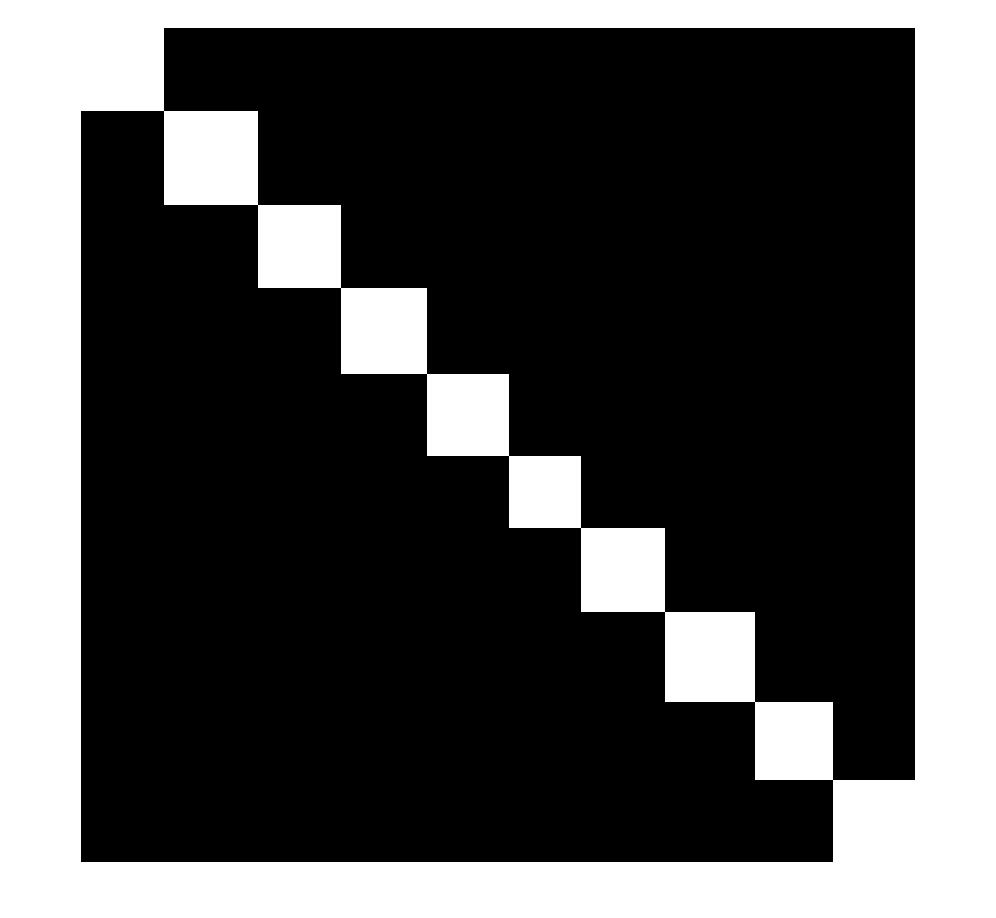
\includegraphics[width=0.3\textwidth]{chap2/k1.jpg}}
	\hspace{1em}
	\bisubcaptionbox{$k=100$下的热力核相似性矩阵}%
					{Affinity matrix of heat kernel with $k=100$}
					[0.3\textwidth]{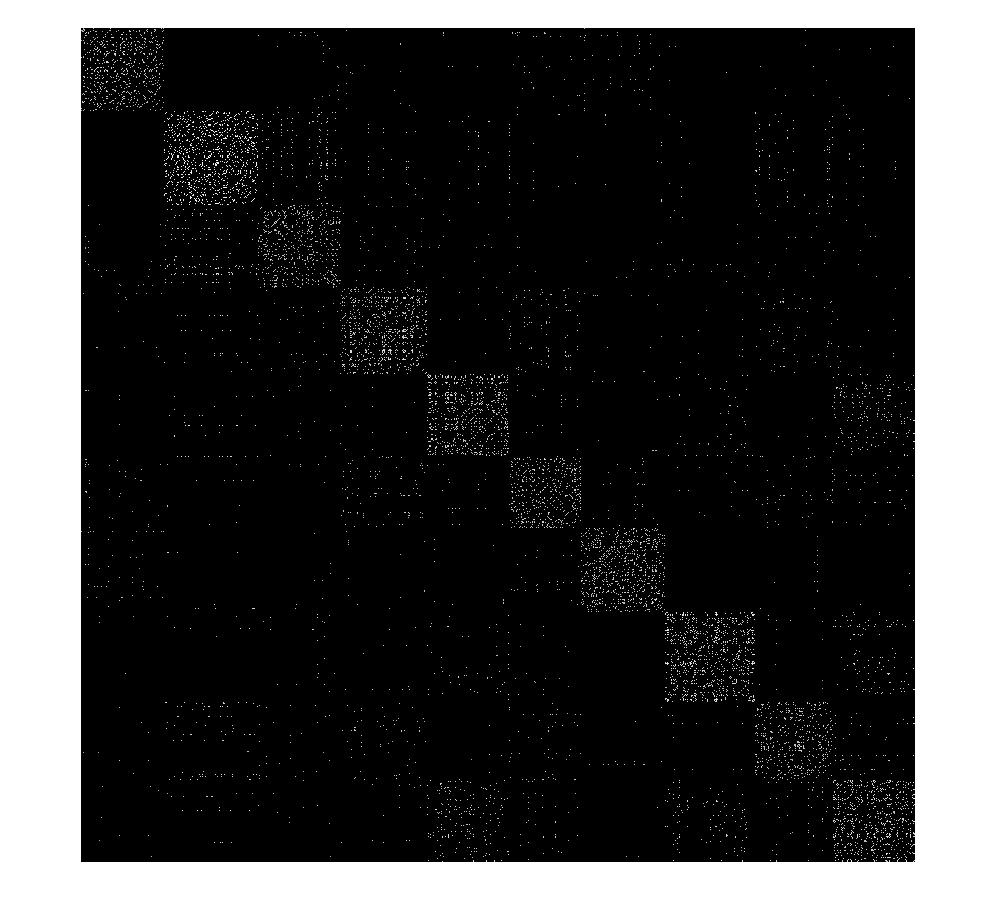
\includegraphics[width=0.3\textwidth]{chap2/k100.jpg}}
	\hspace{1em}
	\bisubcaptionbox{$k=1000$下的热力核相似性矩阵}%
					{Affinity matrix of heat kernel with $k=1000$}%
					[0.3\textwidth]{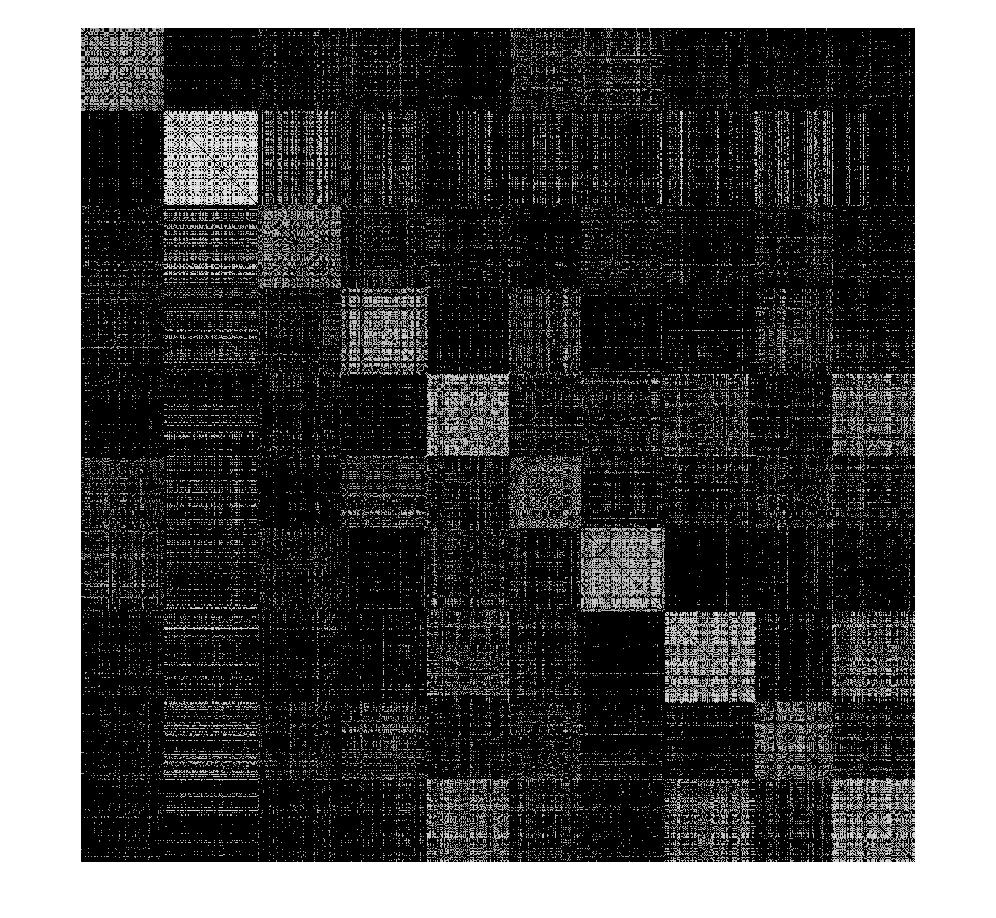
\includegraphics[width=0.3\textwidth]{chap2/k1000.jpg}}
	\bicaption{MNIST子集在理想情况及不同近邻数量$k$下的相似性矩阵}
			  {Ideal affinity matrix and affinity matrices with different neighborhood size $k$ on a subset of MNIST}
  	\label{fig2:affMat}
\end{figure}

本章所提出的方法的目标在于,针对谱聚类的线性近似,在最小的时间消耗下,提取更具有自适应性的相似性信息。这类信息将会更多的考虑局部性保持(locality preserving)这个优化目标,而不仅仅是图像间的距离。受到可扩展谱聚类和数据相似性学习方向上的研究成果\cite{chen2011large,nie2014clustering}的启发,本章提出了一个新颖的自适应相似性矩阵(Adaptive Affinity Matrix,AdaAM)方法。该方法的相似性矩阵相对稠密并可以同时捕捉到全局及局部信息。特别地,AdaAM将相似性矩阵分解成两个相同的低秩矩阵的乘积。作为文献\parencite{ng2002spectral}中描述的理想情况,如果我们假设同一个类内的点对相似性极为相似,则相似性矩阵可能会形成一个低秩矩阵。本算法采用与谱聚类方法相似的优化方法对分解后的矩阵进行优化求解。优化得到的相似性图作为最终结果前的中间态相似性矩阵。通过合并基于热力核获得的$k$-NN相似性图和中间态相似性矩阵,AdaAM采用朴素的谱聚类求解方法计算出一个最终的自适应相似性矩阵。我们将LPP方法作用于此特定的相似性矩阵上进行数据投影,以获得一个用于聚类的距离度量。

在本章中,我们将通过在图像数据集上的聚类实验展示所提出方法的有效性和高效性。第 \ref{sec2:Exp}节通过对本章提出的算法和基于$k$-NN的拉普拉斯特征映\cite{belkin2001laplacian}以及其他最先进方法进行对比展现了AdaAM方法在具有挑战性的数据集上的聚类效果具有明显优势。


\section{自适应相似性矩阵}
在本节中,我们首先对本节采用的数学符号进行说明,其次介绍中间态相似性矩阵的计算方法,然后描述最终自适应相似性矩阵的获取方式,最后对算法流程中的稀疏化策略进行介绍。
\subsection{符号说明}
在本章中,我们以大写英文或希腊字母代表矩阵,小写字母代表向量。所有元素全部为$1$的向量用$\bf{1}$表示。$H$表示中心化矩阵(centering matrix),其定义为:$H = I-\frac{1}{n}\bf{1}\bf{1}^T$。原始数据矩阵以$X \in \mathbb{R}^{n\times d}$表示,其中$n$为数据点的数量,$d$为数据维数。本章中将假设数据矩阵$X$为零均值列归一化矩阵,即$X = HX$。符号$x_i$表示数据矩阵$X$中的第$i$个数据点向量。我们用$A$表示线性投影,相应的距离度量矩阵表示为$M = A^TA$。因此,在该度量矩阵下的距离定义为$dis_m(x_i, x_j) = (x_i - x_j)^TM(x_i - x_j)$。我们将$k$-NN热力核矩阵表示为$W \in \mathbb{R}^{n \times n}$:
\begin{equation}
	w_{ij} = \begin{cases} \mathrm{exp}(-\frac{\|x_i-x_j\|_{2}}{t}), \; &x_i\in\mathcal{N}_k(x_j)\;\mathrm{or}\; x_j\in\mathcal{N}_k(x_i);\\
		0, &\mathrm{otherwise.}\end{cases}          
\end{equation}
此处,$\mathcal{N}_k(x)$表示数据点$x$的 $k$ 个最近邻的集合,我们延续了文献\parencite{niyogi2004locality}中对时间参数$t$的设定。相应的拉普拉斯矩阵表示为$L=D-W$,其中$D$为对角权重矩阵:$d_{ii} = \sum_j w_{ij}$。我们对中间态增量矩阵及最终自适应相似性矩阵都采用$\Delta$表示,相应的对角权重矩阵和拉普拉斯矩阵分别表示为$D_\Delta$和$L_\Delta = D_\Delta-\Delta$。

\subsection{中间态相似性矩阵}
我们将提出的AdaAM算法分为两个部分,分别是中间态相似性矩阵和最终自适应相似性矩阵。本节将对其中的中间态相似性矩阵部分的生成进行介绍。对于第$i$个数据点$x_i$,我们使用相似度$\delta_{ij}$对任意的数据点$x_i$和数据点$x_j$进行连接。由于希望任意两个数据点之间较近的欧氏距离能导致较大的数据点相似度,我们的目标为通过选择最优的相似度$\delta_{ij}$在特定合适的约束下最小化下述的目标函数,
\begin{equation}
	\mathop{\mathrm{min}} \sum_{i,j}^{n} \|x_i-x_j\|_2^2\;\delta_{ij},
\end{equation}
在这里,$\delta_{ij}$表示中间态相似性矩阵$\Delta$中第$ij$个元素。

不同于PCAN算法\cite{nie2014clustering},我们基于图拉普拉斯对该目标函数公式在其约束条件下进行变形,
\begin{equation}
	\mathop{\mathrm{min}}\; tr(X^TL_\Delta X).
	\label{eq2:Delta}
\end{equation}

由于在通常情况下图拉普拉斯为半正定矩阵,因此一个直接又看似可行的思路是将拉普拉斯矩阵分解为两个相同矩阵的乘积。在下文中我们将论述该思路不适用于我们的计算框架。

我们采用$U\in \mathbb{R}^{n\times s}$ 表示一个列正交矩阵,以满足$U^TU = I$,则我们可以假设
\begin{equation}
	L_\Delta = UU^T.
\end{equation}
在对原优化问题进行约束松弛的情况下,我们最终需要求解问题为:
\begin{equation}
	% \begin{split}
		U = \mathop{\mathrm{arg\;min}}_{U^TU=I}\; tr(X^TUU^TX) 
		\Rightarrow U = \mathop{\mathrm{arg\;min}}_{U^TU=I} \;tr(U^TXX^TU)
	% \end{split}
	\label{eq2:simpEigmap}
\end{equation}

如果我们假设矩阵$X$的乘积为矩阵$K$,即$K = XX^T$,则公式(\ref{eq2:simpEigmap})所得为一个简单形式的拉普拉斯特征映射\cite{belkin2001laplacian}。
由此,该优化问题可以通过选择矩阵$K$的多个最小特征值所对应的特征向量形成矩阵进行求解。但是,由于$K$为一个低秩矩阵,一般情况下满足条件$d\ll n$,$K$可以最小化公式(\ref{eq2:simpEigmap})中目标函数的特征向量都存在于数据矩阵$X$的零空间中。
因此,上述问题的最优解不唯一。受LSC(Landmark-based Spectral Clustering)算法\cite{chen2011large}启发,我们将相似性矩阵假设为一个半正定矩阵。不同于对拉普拉斯矩阵进行分解,我们将半正定的相似性矩阵分解为列正交矩阵 $P\in \mathbb{R}^{n\times r}$及其转置矩阵$P^T$的乘积,其中 $r$ 为预期下的矩阵$\Delta$的秩。

由此,我们可以将公式(\ref{eq2:Delta})改写为
\begin{equation}
	% 	\begin{split}
	% 		&\mathop{\mathrm{min}}_{P^TP=I} tr(X^T(D_\Delta-PP^T)X) \\
	% 		&\Rightarrow 
	\mathop{\mathrm{min}}_{P^TP=I} tr(X^TD_\Delta X)+tr(X^T(-PP^T)X),
	% 	\end{split}
	\label{eq2:XLX}
\end{equation}
此处,我们舍弃了连接权重为非负相似度以及图拉普拉斯为半正定矩阵这两个特性。相似性矩阵$\Delta$中的负值连接权重可以用于度量数据点间的不相似度。下面,我们将证明此优化问题的最优解将使$D_\Delta$ 等于 $\bf0$。

\begin{proposition}
	\label{thm2}
	在数据矩阵$X$为列归一化矩阵的条件下,最优化问题(\ref{eq2:XLX})的最优解$P$将使得$D_\Delta=\bf0$成立。
\end{proposition}

\begin{proof}
对于公式(\ref{eq2:XLX})中的第一部分,我们可以将其写为
\begin{equation}
	\begin{split}
		\mathop{\mathrm{min}}\;&\sum_{i=1}^{n} \|x_i\|_2^2\;d_{\Delta ii},\\
		s.t. \;\; &P^TP=I;\\
		&d_{\Delta ii}=(PP^T\textbf{1})_i.
	\end{split}
	\label{eq2:XD}
\end{equation}

令$z=(\|x_1\|_2^2, \|x_2\|_2^2, ... , \|x_n\|_2^2)^T$。此处,取拉格朗日乘子为$\lambda$,公式(\ref{eq2:XD})在一维情况下的优化问题可以表示为
\begin{equation}
	\mathop{\mathrm{min}}\; z^Tpp^T\textbf{1}-\lambda (p^Tp-1)
\end{equation}

最终,最小化优化问题(\ref{eq2:XD})可以被化简为求解问题
\begin{equation}
	\textbf{1}z^Tp=\lambda p
\end{equation}
中最小特征值对应地特征向量。因为矩阵$\textbf{1}z^T$为秩$1$矩阵,所以只存在一个非零特征值$\sum_{i=1}^{n}\|x_i\|_2^2$,同时这也意味着 $\lambda = 0$。由此可知,对于具有任意的小于 $n$的列数且满足优化问题(\ref{eq2:XD})的列正交矩阵$P$,我们可以得出$z^TPP^T\textbf{1}=0$。这个结论等价于
\begin{equation}
	\sum_{i=1}^{n} \|x_i\|_2^2\;d_{\Delta ii} = 0.
\end{equation}

一般性地,对于真实世界数据集中数据点$x_i$,$\|x_i\|_2^2\neq0$恒成立,故能够最小化目标函数(\ref{eq2:XLX})第一部分的最优解$P$ 具有性质$D_\Delta = \textbf{0}$。同时可知,具有性质$D_\Delta = \textbf{0}$的所有$P$的集合构成优化问题(\ref{eq2:XD})的解集。

最小化优化目标函数(\ref{eq2:XLX})的第二部分的矩阵$P$,可以通过求解下述特征问题中最大特征值获得:
\begin{equation}
	\begin{split}
		(XX^T)p = \lambda p
		\Rightarrow {\bf1}XX^Tp = \lambda {\bf1}p
	\end{split}
	\label{eq2:Solu}
\end{equation}

由数据矩阵$X$为零均值列归一化矩阵,可以得知$\lambda {\bf1}p = {\bf1}XX^Tp = 0$。因而,对于大于$0$的最大特征值,其对应地特征向量$p$总满足${\bf1}p = 0$。将令公式(\ref{eq2:XLX})中第二部分取得最小值的解$P$写为 $P=(p_1,p_2,...,p_t)$,可以得到
\begin{equation}
	%\begin{split}
	{\bf1}^T P = {\bf0} \Rightarrow {\bf1}^T PP^T = {\bf0} \Rightarrow d_{\Delta ii} = 0. %\quad(i=1,...,n)
	%\end{split}
\end{equation}
由此可知,特性$D_\Delta = \textbf{0}$对于公式(\ref{eq2:XLX})第二部分的最优解恒成立,并且该最优解属于公式(\ref{eq2:XD})的解集。所以,公式(\ref{eq2:XLX})第二部分的最优解同时可以使目标函数(\ref{eq2:XD})达到最优。完整的优化问题(\ref{eq2:XLX})的最优解使得
\begin{equation}
	D_\Delta={\bf0}。
\end{equation}
\end{proof}

由命题\ref{thm2}可知,优化目标函数(\ref{eq2:XLX})可以进一步化简为
\begin{equation}
	P=\mathop{\mathrm{arg\;max}}_{P^TP=I} \;tr(P^TXX^TP).
	\label{eq2:PXXP}
\end{equation}
公式(\ref{eq2:PXXP})的最优解可以通过对数据矩阵 $X$ 的奇异值分解求得,其运算复杂度依赖于数据维度$d$而不是数据量$n$。至此,我们从同时具有相似度和不相似度信息的原始数据分布中获得了中间态相似性矩阵 $\Delta = PP^T$。矩阵$\Delta$所对应的图拉普拉斯矩阵为$L_\Delta = D_\Delta-\Delta =-\Delta $。

为了能够缓解计算中的噪声影响以及矩阵秩减少的问题,我对矩阵$\Delta$进行了稀疏化处理。我们将在第\ref{sec2:sparse}节对稀疏化处理的细节进行进一步讨论。

\subsection{最终自适应相似性矩阵}
在本节中,我们对朴素的线性谱聚类进行公式化,并且给出最终自适应相似性矩阵的求解方法。

在已经求得中间态相似性矩阵$\Delta$的情况下,我们可以通过求解下述问题获得一个线性投影矩阵$A$:
\begin{equation}
	a = \mathop{\mathrm{arg\;min}}_{a^Ta=1}\; tr(a^TX^T(L+L_\Delta)Xa),
	\label{eq2:AXLXA}
\end{equation}
此处,$a$ 为矩阵$A$的一维情况,且$L+L_\Delta$是$k$-NN热力核与中间态相似性矩阵的拉普拉斯矩阵的组合。投影向量$a$可通过求解特征分解问题的最小特征值得到:
\begin{equation}
	X^T(L-\Delta)Xa = \lambda a
\end{equation}

然后,为在给定$A$的情况下求解公式(\ref{eq2:AXLXA})中的$L_\Delta$,我们依照对公式(\ref{eq2:XLX})的变形,将相似性优化问题进行重写并引入线性投影矩阵$A$:
\begin{equation}
	% \begin{split}		
		P = \mathop{\mathrm{arg\;min}}_{P^TP=I}\; \Big( c+tr(A^TX^TD_\Delta XA) 
		+tr(A^TX^T(-PP^T)XA)\Big),
	% \end{split}
	\label{eq2:AXDXA-PXAAXP}
\end{equation}
这里$c=tr(A^TX^TLXA)$,并且我们假设最终自适应相似性矩阵为$\Delta = PP^T$。由于$X$为列零均值的列归一化矩阵,则$XA$同样为列零均值矩阵,特性$D_\Delta = \textbf{0}$依然成立。由此可知,公式(\ref{eq2:AXDXA-PXAAXP})可化简为
\begin{equation}
	P = \mathop{\mathrm{arg\;max}}_{P^TP=I}\; tr(P^TXAA^TX^TP)
	\label{eq2:PXAAXP}
\end{equation}

公式(\ref{eq2:PXAAXP})可以通过对矩阵$A$进行奇异值分解并提取前$r$个最大奇异值对应的左奇异向量(left-singular vectors)进行求解。我们对从公式(\ref{eq2:PXAAXP})求解得到的自适应相似性矩阵$\Delta=PP^T$进行稀疏化处理,由此可以得到稀疏相似性矩阵。

直观来说,我们可以通过对公式(\ref{eq2:AXLXA})和公式(\ref{eq2:PXAAXP})进行交替迭代求解以使目标函数最小化。然而,如图\ref{fig2:itera}所示,在实际计算中,仅在执行一次迭代运算后所得到的自适应相似性矩阵即可取得很好的聚类效果。持续的迭代求解并没有表现出显著的聚类准确率提升。

在一些算法中图节点的权重具有重要作用,同时例如LPP的一类基于归一化割(Normalized Cuts,NCuts)的方法存在依赖于矩阵$D_\Delta$的优化约束条件。然而在我们的算法中有$D_\Delta = \textbf{0}$,因此,我们将由原始$k$-NN热力核计算得到的权重矩阵$D$叠加到求得的自适应相似性矩阵上,以还原损失的权重信息。最后,我们将原LPP算法中的相似性矩阵替换为由AdaAM方法求得的矩阵$\Delta+D$即可求解出线性投影矩阵$A$ 以及距离度量矩阵$M = A^TA$。

\begin{figure}[t]
	\centering
	\begin{subfigure}{0.49\textwidth}
		\centering
		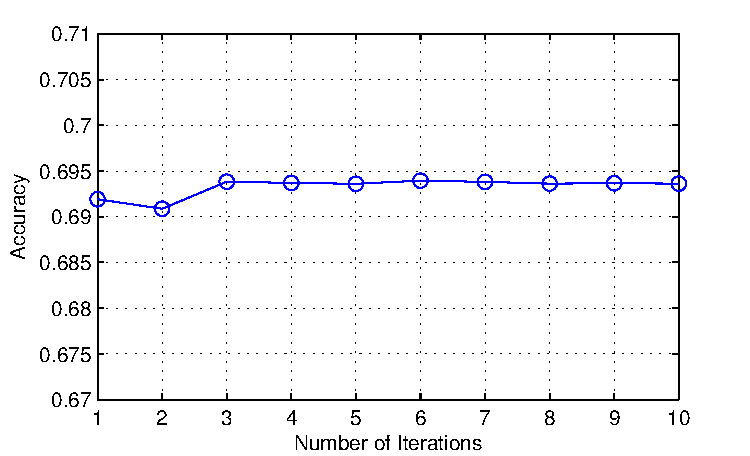
\includegraphics[width=\textwidth]{chap2/itera_data.pdf}
		\caption{}
		\label{fig2:itera}
	\end{subfigure}
	% \hspace{1em}
	\begin{subfigure}{0.49\textwidth}
		\centering
		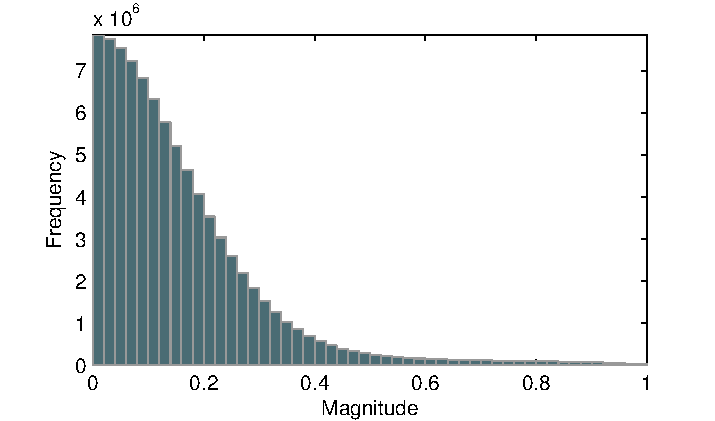
\includegraphics[width=\textwidth]{chap2/delta_hist.pdf}
		\caption{}
		\label{fig2:Hist}
	\end{subfigure}
	\bicaption{a)在数据集USPS上不同的迭代计算次数的聚类效果评价结果。迭代计算所贡献的精度提升小于0.5\%;b)数据集USPS的最终自适应相似性矩阵的元素强度直方图}
			  {a)The evaluation of the clustering performance with different times iterative computation on the data set USPS. The contribution to accuracy made by iteration is less than 0.5\%. b)The histogram of the element magnitude of the final adaptive affinity matrix obtained from data set USPS. }
\end{figure}

\subsection{稀疏化策略}
\label{sec2:sparse}

从优化问题(\ref{eq2:PXXP})和(\ref{eq2:PXAAXP})我们可以观察到,矩阵$XX^T$ 和 $XAA^TX^T$都是低秩矩阵。由于上述的优化问题都需要通过矩阵奇异值分解进行求解,所以这个低秩现象将会导致最优解矩阵$P$的列的数量远小于矩阵 $XX^T$ 和 $XAA^TX^T$ 的秩数。这个计算流程将会产生低秩的相似性矩阵,而低秩相似性矩阵会导致我们的算法中的矩阵秩的进一步减小。为避免该矩阵秩持续减小问题的发生,我们在提出的算法中对矩阵实施了稀疏化操作。我们采用的稀疏化策略可以同时缓解数据图中的噪声边问题。

在图\ref{fig2:Hist}中,我们展示了不经过稀疏化处理情况下通过公式(\ref{eq2:PXAAXP})求得的自适应相似性矩阵的元素强度直方图。从图\ref{fig2:Hist}中我们可以观察到,绝大多数的相似性矩阵元素都集中在数值强度较小的范围内,这有效证明了我们对相似性矩阵进行稀疏化处理的合理性。同时,稀疏化处理可以有效的保留住一部分表达能力更强的相似性元素。

受到$k$-NN热力核构造思路的启发,我们对相似性矩阵$\Delta$中的全部元素根据强度大小进行降序排序,只保留其中的前$s$个元素。假设在稀疏化处理后,仅有类内数据点间的相似性被保留下来,不同类间的数据点相似性被删除。在这种情况下,我们考虑到参数$s$的大小应该与聚类的类数成反比,这可以使最终保留下来元素数量近似与图\ref{fig2:affMat}中所示的理想情况下元素数量保持固定比例。参数$s$的计算公式为:
\begin{equation}
	s = \lfloor \frac{n^2}{\alpha c}\rfloor
\end{equation}
此处 $\lfloor \cdot\rfloor$为向下取整函数,$n^2$为矩阵$\Delta$中的元素总数量,$c$为聚类的类数,$\alpha$为一个可调的比例系数。

\begin{algorithm}[t]
	\SetKwInput{KwData}{输入}
	\SetKwInput{KwResult}{输出}
	\caption{自适应相似性矩阵}
	\label{alg2:AdaAM}
	\KwData{数据点 $X \in \mathbb{R}^{n \times d}$;聚类数量 $c$;近邻数量 $k$;降维后维度 $m$。}
	\KwResult{距离度量矩阵 $M$ 和线性投影矩阵$A$。}
	构建$k$-NN热力核矩阵$W$,相应的对角化权重矩阵$D$ 以及拉普拉斯矩阵$L$。\\
	根据公式(\ref{eq2:PXXP}),计算获得列正交矩阵$P$,并求得相应的中间态相似性矩阵$\Delta = PP^T$。\\
	根据公式(\ref{eq2:AXLXA}),求解得到线性投影矩阵$A$。\\
	求解公式(\ref{eq2:PXAAXP}),构造新的$P$矩阵,生成相应的最终自适应相似性矩阵$\Delta = PP^T$。\\
	通过将LPP算法作用于相似性矩阵$\Delta + D$,计算出线性投影矩阵 $A\in\mathbb{R}^{m\times d}$ 及距离度量矩阵 $M=A^TA$。
\end{algorithm}

对于计算中间态相似性矩阵中的第一次稀疏化处理,我们设置$\alpha$为$2.5$,对于计算最终自适应相似性矩阵中的第二次稀疏化,我们将$\alpha$设置为$5$。此处的$\alpha$通过参数搜索确定,并且能够在大多数数据集上给出稳定的表现。

我们在算法\ref{alg2:AdaAM}中对我们所提出的AdaAM算法流程进行了总结。我们在算法实现中将降维后的维度$m$设置为与聚类的类数相同。


\section{实验结果}
\label{sec2:Exp}
在本节中,我们针对所提出算法在图像数据集上的聚类效果、对构建相似性图中的近邻数量敏感性以及算法的运行时间设计了大量的实验,并与其他最先进的算法进行的对比。实验结果验证了所提出的AdaAM算法的有效性、稳定性和高效性。
\subsection{数据集描述}
我们在五个被广泛使用的灰度图像数据集上对所提出的算法及对照算法进行了性能评估:

\begin{figure}[t]
	\centering
	\bisubcaptionbox{UMIST数据集}%
					{UMIST dataset}
					[0.49\textwidth]{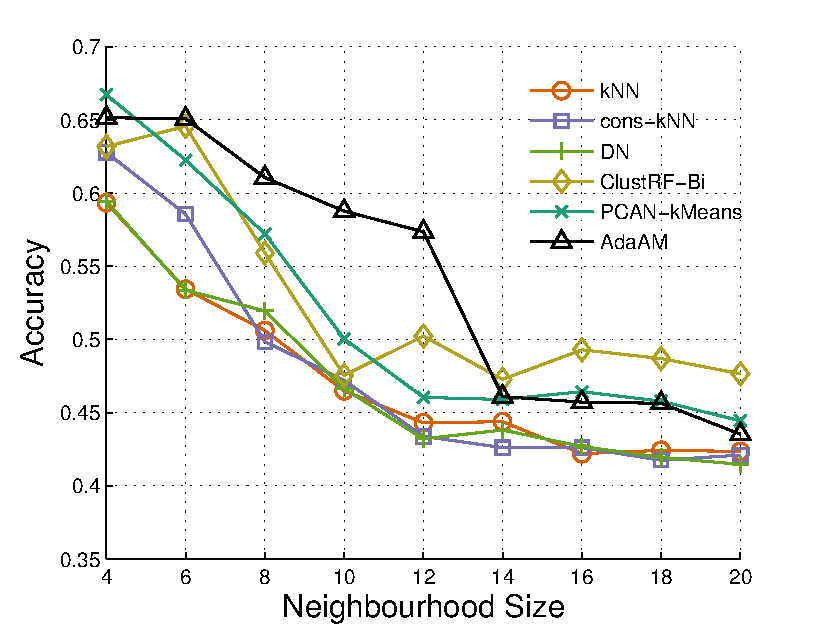
\includegraphics[width=0.49\textwidth]{chap2/sens_UMIST.pdf}}
	\bisubcaptionbox{COIL20数据集}%
					{COIL20 dataset}
					[0.49\textwidth]{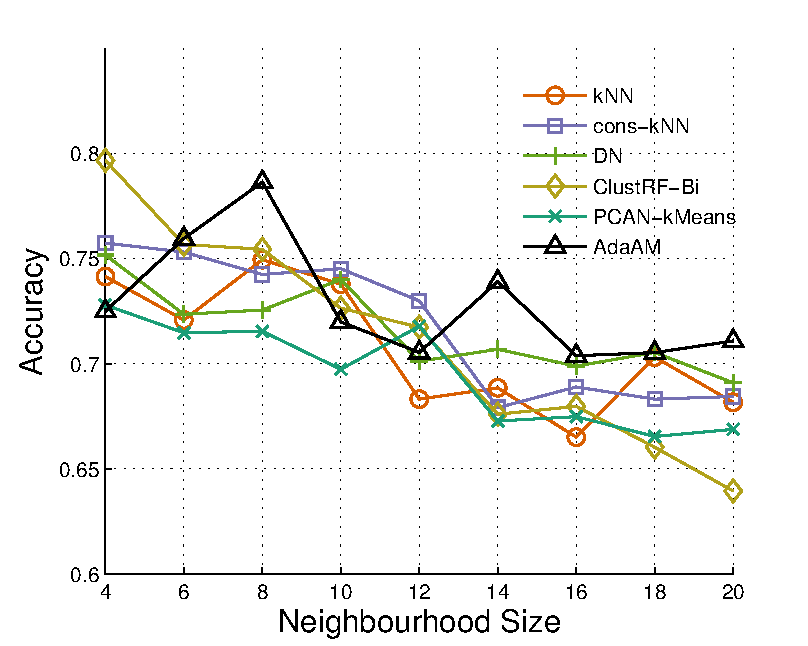
\includegraphics[width=0.49\textwidth]{chap2/sens_COIL20.pdf}}
	\bicaption{在数据集UMIST和COIL20上不同的近邻数量$k$的情况下的算法聚类效果比较}{Clustering results comparison between methods with different neighborhood size $k$ on UMIST and COIL20}
	\label{fig2:Sen}
\end{figure} 

\begin{itemize}
	\item {\textbf{UMIST}}。UMIST人脸数据集 \cite{graham1998characterising}包括20个人的共计575张灰度图片,每张图片尺寸为220$ \times $220像素。在我们的实验中,我们将原图缩小到40$ \times $40像素。
	\item {\textbf{COIL20}}。COIL20数据集\cite{nene1996columbia}包含20各不同物体,共1,440张灰度图片。数据集图片尺寸为32$\times$32像素,图片背景被丢弃仅保留了前景物体。
	\item {\textbf{USPS}}。USPS手写数字数据库\cite{hull1994database}包含了10个数字共计9,298张的灰度图像,图像尺寸为16$\times$16像素。
	\item {\textbf{MNIST}}。MNIST手写数字数据库\cite{lecun1998gradient}训练集包含10类数字共计70,000张灰度图像。图片尺寸为28$\times$28像素。在我们的实验中,我们使用了该数据库训练集中前10,000张图片。
	\item {\textbf{ExYaleB}}。Extended Yale Face Database B(ExYaleB)人脸数据集\cite{KCLee05}由2,414张经过裁剪的人脸图像组成,包含38个个体,每个个体在不同光照下拍摄大约64张图像。在实验中,我们将ExYaleB图像缩小到32$ \times $32像素。
\end{itemize}

在表格\ref{tab2:Data}中,我们总结了五个基准图像数据集的统计量描述。

\begin{table}[t]
	\bicaption{五个基准数据集的统计量描述}{Statistics of five benchmark data sets}
	\label{tab2:Data}
	\centering
		%\begin{sc}
	\begin{tabular}{l c c c}
		\toprule
		数据集 & 实例数目 & 特征维度 & 类别数目\\ 
		\midrule
		UMIST & 575 & 1,600 & 20\\
		COIL20 & 1,440 & 1,024 & 20\\
		USPS & 9,298 & 256 & 10\\
		MNIST & 10,000 & 784 & 10\\
		ExYaleB & 2,414 & 1,024 & 38\\
		\bottomrule
	\end{tabular}
		%\end{sc}
\end{table}

\subsection{对照算法介绍}
我们将所提出的AdaAM方法的聚类效果与本节中介绍的其他相似性学习算法进行了比较。 我们将LPP方法分别应用于通过这些最先进方法生成的相似性矩阵,以获取距离度量矩阵。

\begin{itemize}
	\item \textbf{Con-$k$NN}。Consensus $k$-NNs(Cons-$k$NN)算法\cite{premachandran2013consensus}的目标在于选取更鲁棒的数据点近邻集合。Cons-$k$NN方法通过收集多轮$k$-NN相似性计算中的共识信息,来为数据点近邻集合的选择提供判断标准。
	\item \textbf{DN}。Dominant Neighborhoods(DN)算法\cite{pavan2007dominant}通过在已构建出的相似性图中迭代地选取最大团的方法,实现对相似性矩阵中存在的噪声边的过滤。
	\item \textbf{ClustRF-Bi}。ClustRF-Bi算法\cite{criminisi2012decision,pei2013unsupervised}是ClustRF-Strct \cite{zhu2014constructing}算法的一个计算量较小的特例。由于原始ClustRF-Strct算法在仅有数千个数据实例的情况就需要极大量的计算机内存,我们在本章的实验中采用了这个计算量和内存需求相对可行的特例。ClustRF-Strct提出了一种具有结构感知能力的相似性推断模型,该模型通过利用随机森林进行聚类从而构建数据的相似性图。ClustRF-Bi作为一个特例仅通过随机森林聚类构建二值化的相似性矩阵。
	\item \textbf{PCAN}。文献\parencite{nie2014clustering}提出了Projected Clustering with Adaptive Neighbors(PCAN)方法。由于PCAN是一种可以同时生成线性投影和聚类的算法,所以在结果展示中,我们将PCAN的投影和$k$-means聚类的组合方法表示为PCAN-$k$Means方法,并在表格\ref{tab2:Acc}中显示仅采用PCAN算法生成的聚类结果以供对照参考。
	\item \textbf{$k$-NN}。我们还将所提出的方法与采用$k$-NN热力核相似性矩阵直接进行线性投影的效果进行比较,即采用$k$-NN热力核的LPP算法。我们在后续实验中使用$k$-NN表示这种典型的方法。
\end{itemize}

\begin{figure}[t]
	\centering
	\bisubcaptionbox{USPS数据集}%
					{USPS dataset}
					[0.49\textwidth]{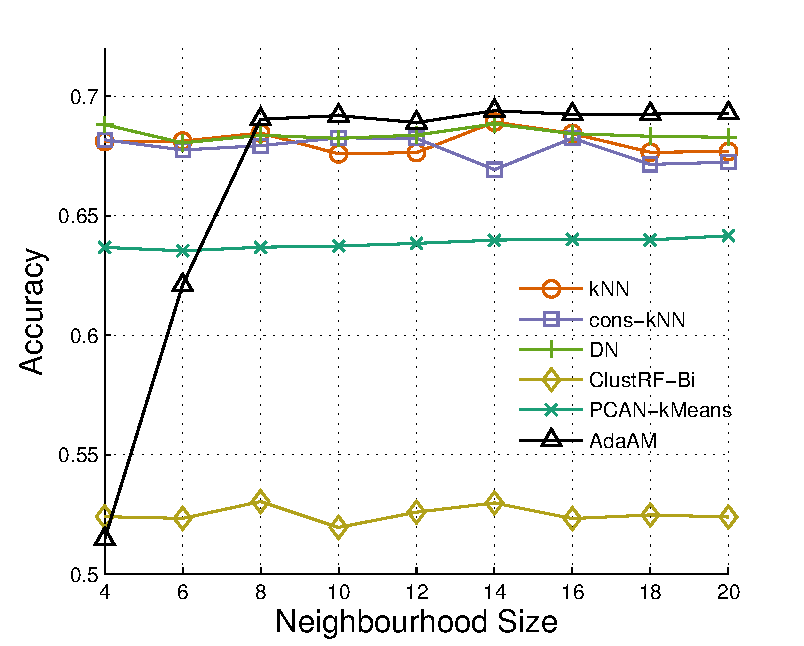
\includegraphics[width=0.49\textwidth]{chap2/sens_USPS.pdf}}
	\bisubcaptionbox{MNIST数据集}%
					{MNIST dataset}
					[0.49\textwidth]{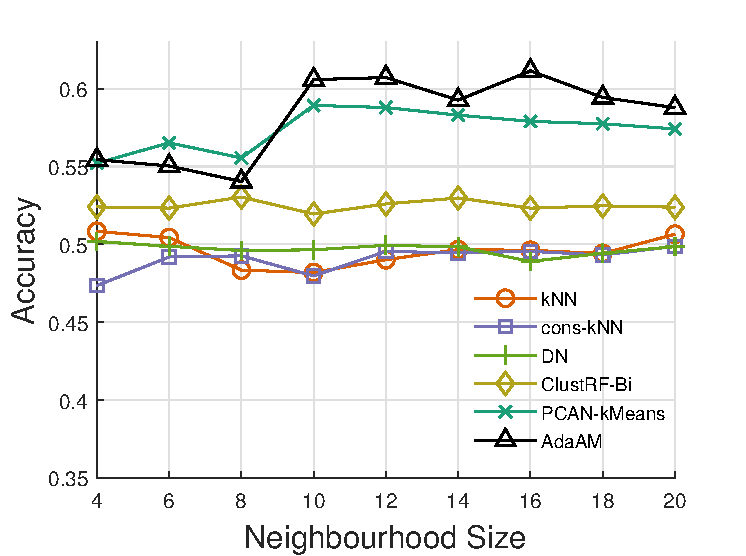
\includegraphics[width=0.49\textwidth]{chap2/sens_MNIST.pdf}}
	\bicaption{在数据集USPS和MNIST上不同的近邻数量$k$的情况下的算法聚类效果比较}{Clustering results comparison between methods with different neighborhood size $k$ on USPS and MNIST}
	\label{fig2:Sen2}
\end{figure} 
\begin{table}[t]
	\bicaption{不同图像数据集上的聚类准确率(\%)}
	{Clustering accuracy on different image datasets(\%)}
	\label{tab2:Acc}
	\centering
	% \begin{small}
		%\begin{sc}
		\begin{tabular}{llccccccc}
			\toprule
			& &$k$-NN &Cons-$k$NN &DN &ClustRF-Bi &PCAN-$k$Means &PCAN& AdaAM
			\\
			\midrule
			\multirow{2}{*}{UMIST} & Avg & 58.16& 60.27& 59.15& 64.63& 53.79& \multirow{2}{*}{55.30}   & \textbf{66.06}\\
			& Max& 65.39& 69.22& 66.96& 74.44& 56.52&& \textbf{75.65}\\
			\midrule
			\multirow{2}{*}{COIL20} & Avg & 71.89& 75.53& 71.95& \textbf{76.50}& 72.28& \multirow{2}{*}{81.74}& 74.72\\
			& Max& 81.18& 84.31& 82.01& 85.07& 83.75&& \textbf{87.29}\\
			\midrule
			\multirow{2}{*}{USPS}  & Avg & 68.25& 68.21& 68.08& 58.74& 64.04& \multirow{2}{*}{64.20}  & \textbf{69.36}\\
			& Max& 68.35& 68.34& 68.31& 65.90& 67.95&& \textbf{69.61}\\
			\midrule
			\multirow{2}{*}{MNIST} & Avg & 48.13& 47.88& 49.72& 51.93& 58.93& \multirow{2}{*}{59.83}  & \textbf{60.84}\\
			& Max& 48.27& 48.00& 49.76& 52.03& 58.98&& \textbf{61.34}\\
			\midrule
			\multirow{2}{*}{ExYaleB} & Avg& 24.17& 25.63& 24.21& 23.10& 25.74& \multirow{2}{*}{25.89} & \textbf{54.36}\\
			& Max& 26.76& 28.75& 27.42& 26.43& 27.63&& \textbf{57.87}\\
			\bottomrule
		\end{tabular}
		%\end{sc}
	% \end{small}
\end{table}

\subsection{参数选择与实验设置}
由于在无监督学习任务中不存在验证数据集,所以为了实现更一般化的参数选择情况,我们对实验中的所有算法采用了相同的参数选择标准。我们将每个数据实例的近邻数量设置为$k = \mathrm{Round}(\mathrm{log}_2\frac{n}{c})$,其中$n$为数据实例数量,$c$为类别数量,$Round(x)=\lfloor x+\frac{1}{2}\rfloor$。我们参考文献\parencite{ng2002spectral}的结论,将投影的维度设置为与类别数目相同,即距离度量矩阵的秩与类别数相同。所提出的算法中的其他参数在所有实验中均固定不变。

我们将10次独立重复的$k$-means聚类表示为1轮聚类,并在每轮所有结果中选择类内和最小的结果作为该轮$k$-means的聚类结果。在进行聚类性能评估中,我们对每种算法分别应用100轮$k$-means聚类用于(参见表\ref{tab2:Acc})。在近邻数量$k$的敏感性实验中,我们应用10轮$k$-means聚类(参见图\ref{fig2:Sen},图\ref{fig2:Sen2}和图\ref{fig2:Sen3}),而在运行时间测试实验中,我们仅进行一轮$k$-means聚类(参见图\ref{fig2:Time})。


\begin{figure}[t]
	\centering
	\bisubcaptionbox{ExYaleB数据集}%
					{ExYaleB dataset}
					[0.9\textwidth]{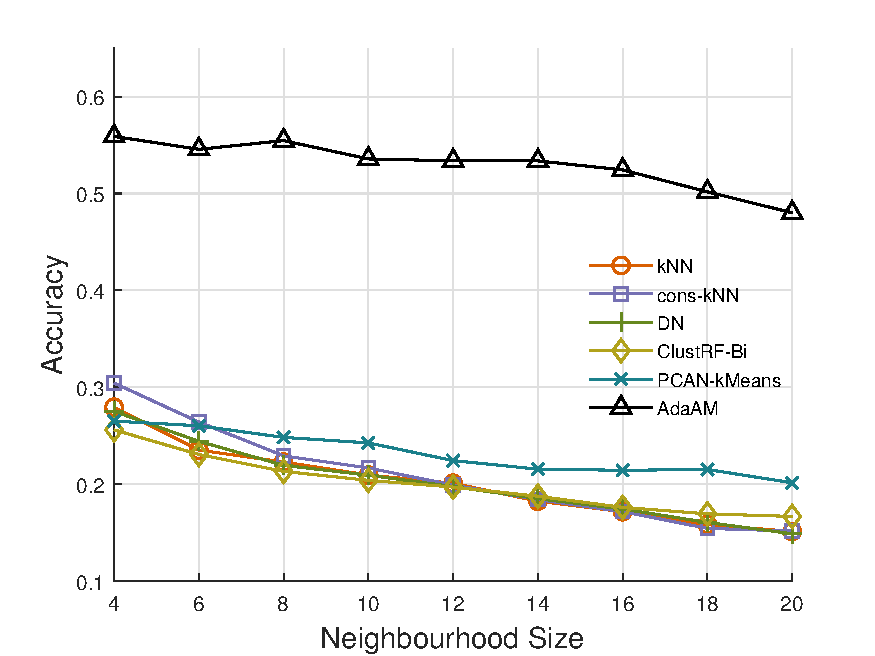
\includegraphics[width=0.9\textwidth]{chap2/sens_ExYaleB1.pdf}}
	\bicaption{在数据集ExYaleB上不同的近邻数量$k$的情况下的算法聚类效果比较}{Clustering results comparison between methods with different neighborhood size $k$ on ExYaleB}
	\label{fig2:Sen3}
\end{figure} 
在聚类效果评估中,我们通过将获得的聚类标签与数据集的真实标注进行比较,使用准确率(accuracy,Acc)来衡量性能。准确率定义如下:
\begin{equation}
	\mathrm{Acc} = \frac{1}{n}\sum^{n}_{i=1}\delta(p_i, map(q_i))
\end{equation}
其中$n$为数据实例数量,$p_i$是数据$x_i$的预测标签,$q_i$为真实标签。当$x=y$时$\delta(x, y) = 1$,否则$\delta(x,y) = 0$。$map(q_i)$表示最佳匹配函数,该函数通过在预测出的类之间交换类标签实现,预测标签与真实标签的最佳匹配。

全部实验都通过MATLAB R2014a实现,并运行在具有Quad Core 3.00 GHz CPU和16 GB内存的Linux系统计算机上。

\subsection{性能评估与比较}
\begin{figure}[t]
	\centering
	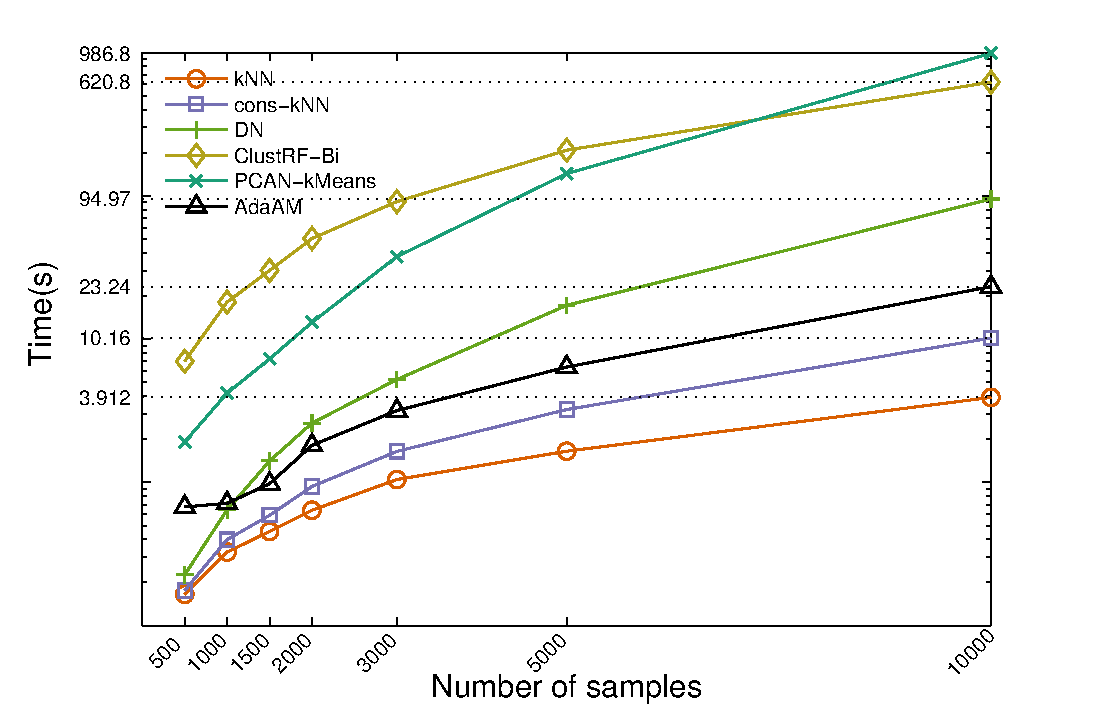
\includegraphics[width=0.9\columnwidth]{chap2/time.pdf}
	\bicaption{不同数据实例数量的情况下六个算法的时间使用比较}{Time consumption of six approaches with different number of data instances}
	\label{fig2:Time}
\end{figure}

在聚类准确率评估的实验中,我们在上述五个基准数据集上对提出的AdaAM方法及其他五种算法进行了数据投影效果的评估。表\ref{tab2:Acc}给出每个模型在100轮$k$-means聚类中聚类预测准确率的平均值和最大值。由于PCAN算法不通过$k$-means聚类而直接产生聚类结果,所有PCAN性能评估结果仅有唯一结果,不存在平均值与最大值。从表\ref{tab2:Acc}中我们可以观察到AdaAM算法在无监督度量学习任务上的优越性。在绝大多数情况下,AdaAM算法的性能明显优于其他方法。我们的方法在五个数据集的平均准确率指标上获得了四个最优,在最大准确率指标上五个全部最优。我们还可以观察到,所提出的AdaAM在ExYaleB数据集上相对其他五种方法具有绝对性优势。与其他数据集不同,ExYaleB中的图像数据已针对人脸进行了较好地对齐,并图片拍摄场景处于不同的光照环境下。这种差异使得相同光照下的图片即使属于不同类别的图像依然具有较大的相似度,从而使数据图上类间连接增多,导致了高秩的相似性矩阵。我们的方法基于最优相似性矩阵的低秩近似,能够有效处理相似性矩阵中的此类噪声。

由于在准确率评估实验中近邻数量$k$选择标准是固定的,这可能会导致算法无法在实验中获得最优性能。因此我们在图\ref{fig2:Sen}、图\ref{fig2:Sen2}及图\ref{fig2:Sen3}中展示了AdaAM与对照算法在五个图像数据上的聚类准确率随近邻数量大小变化的趋势。我们在每个数据集上分别设计了近邻数量从$k=4$到$k=20$、间隔为2的9组实验,以评估不同算法的聚类效果是否会随近邻数量不同,即相似性矩阵的稀疏程度,而产生显著的波动。从图中可以看出,在大多数情况下,AdaAM可取得最佳性能,并且对近邻数量的敏感性与其他模型相当或更低。由于我们的方法基于最佳相似性矩阵的低秩近似,需要更多的成对相似度的信息。因此,对于极小的近邻数量$k$,部分基线方法有时比我们的方法效果更好,这一点可以从图\ref{fig2:Sen2}可以看出。

在图\ref{fig2:Time}中,我们通过半对数图描绘了六种算法在不同数据量的MNIST子集上的运行时间,以此说明AdaAM方法的高效性。 从图中可以看出,我们的方法在实际使用中是一种时间代价较低的算法。相比于PCAN-$k$Means,ClustRF-Bi和DN方法,AdaAM算法的时间消耗要低得多。需要注意的是,$k$-NN作为一个基线算法,本身并不需要进行相似性矩阵学习,因此其所需的运行时间仅包括$k$-NN热力核相似性矩阵构建、LPP线性投影矩阵计算及$k$-means聚类这三种所有对照算法共享的基本操作,所以其计算效率必然最高。我们同时还展示了AdaAM的运行时间大约为Cons-$k$NN的两倍,但整体性能性能要好得多。

\section{本章小结}
在本章中,我们提出了一种用于无监督度量学习的创新性的的相似性学习方法,称为自适应相似性矩阵矩阵(Adaptive Affinity Matrix,AdaAM)。在我们所提出的新的相似性学习模型中,相似性矩阵是从与谱聚类相同的计算框架中学习获得的。 更具体地说,我们表明相似性学习可以简化为奇异值分解问题。获得学习到的相似性矩阵后,可以借助于类似LPP这样基于相似性图的现成的算法来学习距离度量。我们所采用的低秩近似的优化方法可以在相似性矩阵学习的过程中进一步提高学习效率。
我们在UMIST、COIL20、USPS、MNIST及ExYaleB五个被广泛使用的图像数据集上对AdaAM及其他对照算法的进行了大量聚类实验。
实验结果证明了所提出的方法AdaAM的性能优越性、稳定性与高效性。
% !TEX root = ../thesis.tex

\chapter{简介}

这是 \sjtuthesis 的示例文档,基本上覆盖了模板中所有格式的设置。建议大家在使用模
板之前,除了阅读《\sjtuthesis\ 使用文档》,这个示例文档也最好能看一看。

\section{二级标题}

\subsection{三级标题}

\subsubsection{四级标题}

Lorem ipsum dolor sit amet, consectetur adipiscing elit, sed do eiusmod tempor
incididunt ut labore et dolore magna aliqua. Ut enim ad minim veniam, quis
nostrud exercitation ullamco laboris nisi ut aliquip ex ea commodo consequat.
Duis aute irure dolor in reprehenderit in voluptate velit esse cillum dolore eu
fugiat nulla pariatur. Excepteur sint occaecat cupidatat non proident, sunt in
culpa qui officia deserunt mollit anim id est laborum.

\section{脚注}

Lorem ipsum dolor sit amet, consectetur adipiscing elit, sed do eiusmod tempor
incididunt ut labore et dolore magna aliqua. \footnote{Ut enim ad minim veniam,
quis nostrud exercitation ullamco laboris nisi ut aliquip ex ea commodo
consequat. Duis aute irure dolor in reprehenderit in voluptate velit esse cillum
dolore eu fugiat nulla pariatur.}

\section{字体}


上海交通大学是我国历史最悠久的高等学府之一,是教育部直属、教育部与上海市共建的全
国重点大学,是国家“七五”、“八五”重点建设和“211 工程”、“985 工程”的首批建
设高校。经过 115 年的不懈努力,上海交通大学已经成为一所“综合性、研究型、国际化”
的国内一流、国际知名大学,并正在向世界一流大学稳步迈进。 

{\songti 十九世纪末,甲午战败,民族危难。中国近代著名实业家、教育家盛宣怀和一批
  有识之士秉持“自强首在储才,储才必先兴学”的信念,于 1896 年在上海创办了交通大
  学的前身——南洋公学。建校伊始,学校即坚持“求实学,务实业”的宗旨,以培养“第
  一等人才”为教育目标,精勤进取,笃行不倦,在二十世纪二三十年代已成为国内著名的
  高等学府,被誉为“东方MIT”。抗战时期,广大师生历尽艰难,移转租界,内迁重庆,
  坚持办学,不少学生投笔从戎,浴血沙场。解放前夕,广大师生积极投身民主革命,学校
  被誉为“民主堡垒”。}

{\heiti 新中国成立初期,为配合国家经济建设的需要,学校调整出相当一部分优势专业、
  师资设备,支持国内兄弟院校的发展。五十年代中期,学校又响应国家建设大西北的号
  召,根据国务院决定,部分迁往西安,分为交通大学上海部分和西安部分。1959 年 3月
  两部分同时被列为全国重点大学,7 月经国务院批准分别独立建制,交通大学上海部分启
  用“上海交通大学”校名。历经西迁、两地办学、独立办学等变迁,为构建新中国的高等
  教育体系,促进社会主义建设做出了重要贡献。六七十年代,学校先后归属国防科工委和
  六机部领导,积极投身国防人才培养和国防科研,为“两弹一星”和国防现代化做出了
  巨大贡献。}

{\kaishu 改革开放以来,学校以“敢为天下先”的精神,大胆推进改革:率先组成教授代
  表团访问美国,率先实行校内管理体制改革,率先接受海外友人巨资捐赠等,有力地推动
  了学校的教学科研改革。1984 年,邓小平同志亲切接见了学校领导和师生代表,对学校
  的各项改革给予了充分肯定。在国家和上海市的大力支持下,学校以“上水平、创一流”
  为目标,以学科建设为龙头,先后恢复和兴建了理科、管理学科、生命学科、法学和人文
  学科等。1999 年,上海农学院并入;2005 年,与上海第二医科大学强强合并。至此,学
  校完成了综合性大学的学科布局。近年来,通过国家“985 工程”和“211 工程”的建
  设,学校高层次人才日渐汇聚,科研实力快速提升,实现了向研究型大学的转变。与此同
  时,学校通过与美国密西根大学等世界一流大学的合作办学,实施国际化战略取得重要突
  破。1985 年开始闵行校区建设,历经 20 多年,已基本建设成设施完善,环境优美的现
  代化大学校园,并已完成了办学重心向闵行校区的转移。学校现有徐汇、闵行、法华、七
  宝和重庆南路(卢湾)5 个校区,总占地面积 4840 亩。通过一系列的改革和建设,学校
  的各项办学指标大幅度上升,实现了跨越式发展,整体实力显著增强,为建设世界一流大
  学奠定了坚实的基础。}

{\fangsong 交通大学始终把人才培养作为办学的根本任务。一百多年来,学校为国家和社
  会培养了 20余万各类优秀人才,包括一批杰出的政治家、科学家、社会活动家、实业
  家、工程技术专家和医学专家,如江泽民、陆定一、丁关根、汪道涵、钱学森、吴文俊、
  徐光宪、张光斗、黄炎培、邵力子、李叔同、蔡锷、邹韬奋、陈敏章、王振义、陈竺等。
  在中国科学院、中国工程院院士中,有 200 余位交大校友;在国家 23 位“两弹一星”
  功臣中,有 6 位交大校友;在 18 位国家最高科学技术奖获得者中,有 3 位来自交大。
  交大创造了中国近现代发展史上的诸多“第一”:中国最早的内燃机、最早的电机、最早
  的中文打字机等;新中国第一艘万吨轮、第一艘核潜艇、第一艘气垫船、第一艘水翼艇、
  自主设计的第一代战斗机、第一枚运载火箭、第一颗人造卫星、第一例心脏二尖瓣分离
  术、第一例成功移植同种原位肝手术、第一例成功抢救大面积烧伤病人手术等,都凝聚着
  交大师生和校友的心血智慧。改革开放以来,一批年轻的校友已在世界各地、各行各业崭
  露头角。}

{\ifcsname lishu\endcsname\lishu\else[无 \cs{lishu} 字体。]\fi 截至 2011 年 12
  月 31 日,学校共有 24 个学院 / 直属系(另有继续教育学院、技术学院和国际教育学
  院),19 个直属单位,12 家附属医院,全日制本科生 16802 人、研究生24495 人(其
  中博士研究生 5059 人);有专任教师 2979 名,其中教授 835 名;中国科学院院士 15
  名,中国工程院院士 20 名,中组部“千人计划”49 名,“长江学者”95 名,国家杰出
  青年基金获得者 80 名,国家重点基础研究发展计划(973 计划)首席科学家 24名,国
  家重大科学研究计划首席科学家 9名,国家基金委创新研究群体 6 个,教育部创新团队
  17 个。}

{\ifcsname youyuan\endcsname\youyuan\else[无 \cs{youyuan} 字体。]\fi 学校现有本
  科专业 68 个,涵盖经济学、法学、文学、理学、工学、农学、医学、管理学和艺术等九
  个学科门类;拥有国家级教学及人才培养基地 7 个,国家级校外实践教育基地 5个,国
  家级实验教学示范中心 5 个,上海市实验教学示范中心 4 个;有国家级教学团队 8个,
  上海市教学团队 15 个;有国家级教学名师 7 人,上海市教学名师 35 人;有国家级精
  品课程 46 门,上海市精品课程 117 门;有国家级双语示范课程 7 门;2001、2005 和
  2009 年,作为第一完成单位,共获得国家级教学成果 37 项、上海市教学成果 157
  项。}

% !TeX root = ../thesis.tex

\chapter{浮动体}

\section{插图}

插图功能是利用 \TeX\ 的特定编译程序提供的机制实现的,不同的编译程序支持不同的图
形方式。有的同学可能听说“\LaTeX\ 只支持 EPS”,事实上这种说法是不准确的。\XeTeX
可以很方便地插入 EPS、PDF、PNG、JPEG 格式的图片。

一般图形都是处在浮动环境中。之所以称为浮动是指最终排版效果图形的位置不一定与源文
件中的位置对应,这也是刚使用 \LaTeX\ 同学可能遇到的问题。如果要强制固定浮动图形
的位置,请使用 \pkg{float} 宏包,它提供了 \texttt{[H]} 参数。

\subsection{单个图形}

图要有图题,研究生图题采用中英文对照,并置于图的编号之后,图的编号和图题应置于图
下方的居中位置。引用图应在图题右上角标出文献来源。当插图中组成部件由数字或字母等
编号表示时,可在插图下方添加图注进行说明,如图~\ref{fig:cn_100t} 所示。

\begin{figure}[!htp]
  \centering
  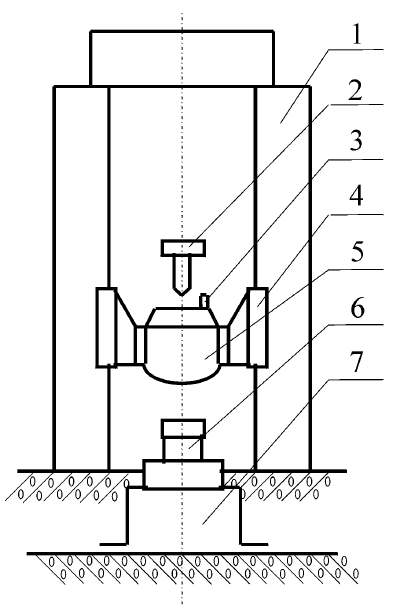
\includegraphics[width=4cm]{cn_100t.png} \\
    1.立柱 2.提升释放机构 3.标准冲击加速度计 \\
    4.导轨 5.重锤 6.被校力传感器 7.底座 \\
  \bicaption[出现在插图索引中]
    {单个图形示例\cite{he1999}。如果表格的标题很长,那么在表格索引中就会很不美观。可
      以在前面用中括号写一个简短的标题,这个标题会出现在索引中。}
    {Stay hungry, stay foolish.}
 \label{fig:cn_100t}
\end{figure}

Lorem ipsum dolor sit amet, consectetur adipisici elit, sed do eiusmod tempor
incididunt ut labore et dolore magna aliqua. Ut enim ad minim veniam, quis
nostrud exercitation ullamco laboris nisi ut aliquip ex ea commodo consequat.
Duis aute irure dolor in reprehenderit in voluptate velit esse cillum dolore eu
fugiat nulla pariatur. Excepteur sint occaecat cupidatat non proident, sunt in
culpa qui officia deserunt mollit anim id est laborum.

\subsection{多个图形}

简单插入多个图形的例子如图~\ref{fig:SRR} 所示。这两个水平并列放置的子图共用一个
图形计数器,没有各自的子图题。

\begin{figure}[!htp]
  \centering
  
\includegraphics[height=2cm]{sjtu-badge.pdf}
  \hspace{1cm}
  
\includegraphics[height=2cm]{sjtu-badge.pdf}
  \bicaption{中文题图}{English caption}
  \label{fig:SRR}
\end{figure}

如果多个图形相互独立,并不共用一个图形计数器,那么用 \texttt{minipage} 或者
\texttt{parbox} 就可以,如图~\ref{fig:parallel1} 与图~\ref{fig:parallel2}。

\begin{figure}[!htp]
\begin{minipage}{0.48\textwidth}
  \centering
  
\includegraphics[height=1.5cm]{sjtu-name.pdf}
  \caption{并排第一个图}
  \label{fig:parallel1}
\end{minipage}\hfill
\begin{minipage}{0.48\textwidth}
  \centering
  
\includegraphics[height=1.5cm]{sjtu-name.pdf}
  \caption{并排第二个图}
  \label{fig:parallel2}
\end{minipage}
\end{figure}

Lorem ipsum dolor sit amet, consectetur adipisici elit, sed do eiusmod tempor
incididunt ut labore et dolore magna aliqua. Ut enim ad minim veniam, quis
nostrud exercitation ullamco laboris nisi ut aliquip ex ea commodo consequat.
Duis aute irure dolor in reprehenderit in voluptate velit esse cillum dolore eu
fugiat nulla pariatur. Excepteur sint occaecat cupidatat non proident, sunt in
culpa qui officia deserunt mollit anim id est laborum.

如果要为共用一个计数器的多个子图添加子图题,建议使用较新的 \pkg{subcaption}宏
包,不建议使用 \pkg{subfigure} 或 \pkg{subfig} 等宏包。

推荐使用 \pkg{subcaption} 宏包的 \cs{subcaptionbox} 并排子图,子图题置于子图之
下,子图号用 a)、b) 等表示。也可以使用 \pkg{subcaption} 宏包的 \cs{subcaption}
(放在 minipage中,用法同 \cs{caption})。

搭配 \pkg{bicaption} 宏包时,可以启用 \cs{subcaptionbox} 和 \cs{subcaption} 的双
语变种 \cs{bisubcaptionbox} 和 \cs{bisubcaption},如图~\ref{fig:bisubcaptionbox}
所示。

\begin{figure}[!hbtp]
  \centering
  \bisubcaptionbox{$R_3 = 1.5\text{mm}$ 时轴承的压力分布云图}%
                  {Pressure contour of bearing when $R_3 = 1.5\text{mm}$}%
                  [6.4cm]{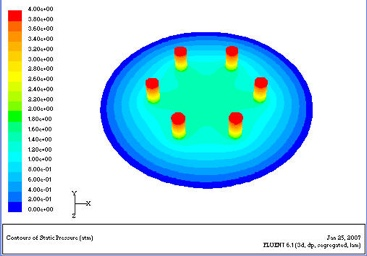
\includegraphics[height=2.5cm]{pressure15.jpg}}
  \hspace{1cm}
  \bisubcaptionbox{$R_3 = 2.5\text{mm}$ 时轴承的压力分布云图}%
                  {Pressure contour of bearing when $R_3 = 2.5\text{mm}$}%
                  [6.4cm]{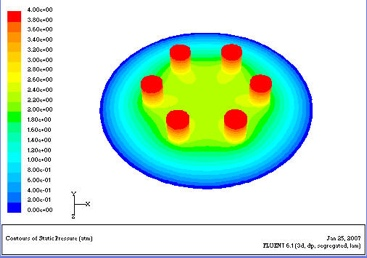
\includegraphics[height=2.5cm]{/pressure25.jpg}}
  \bicaption{包含子图题的范例(使用 subcaptionbox)}
            {Example with subcaptionbox}
  \label{fig:bisubcaptionbox}
\end{figure}

\pkg{subcaption} 宏包也提供了 \pkg{subfigure} 和 \pkg{subtable} 环境,如
图~\ref{fig:subfigure}。

\begin{figure}[!htp]
  \centering
  \begin{subfigure}{0.3\textwidth}
    \centering
    
\includegraphics[height=2cm]{sjtu-badge.pdf}
    \caption{校徽}
  \end{subfigure}
  \hspace{1cm}
  \begin{subfigure}{0.4\textwidth}
    \centering
    
\includegraphics[height=1.5cm]{sjtu-name.pdf}
    \caption{校名。注意这个图略矮些,subfigure 中同一行的子图在顶端对齐。}
  \end{subfigure}
  \caption{包含子图题的范例(使用 subfigure)}
  \label{fig:subfigure}
\end{figure}

Lorem ipsum dolor sit amet, consectetur adipisici elit, sed do eiusmod tempor
incididunt ut labore et dolore magna aliqua. Ut enim ad minim veniam, quis
nostrud exercitation ullamco laboris nisi ut aliquip ex ea commodo consequat.
Duis aute irure dolor in reprehenderit in voluptate velit esse cillum dolore eu
fugiat nulla pariatur. Excepteur sint occaecat cupidatat non proident, sunt in
culpa qui officia deserunt mollit anim id est laborum.

\section{表格}

\subsection{基本表格}

编排表格应简单明了,表达一致,明晰易懂,表文呼应、内容一致。表题置于表上,研究生
学位论文可以用中、英文两种文字居中排写,中文在上,也可以只用中文。

表格的编排建议采用国际通行的三线表\footnote{三线表,以其形式简洁、功能分明、阅读
方便而在科技论文中被推荐使用。三线表通常只有 3 条线,即顶线、底线和栏目线,没有
竖线。}。三线表可以使用 \pkg{booktabs} 提供的 \cs{toprule}、\cs{midrule} 和
\cs{bottomrule}。它们与 \pkg{longtable} 能很好的配合使用。

\begin{table}[!hpt]
  \caption[一个颇为标准的三线表]{一个颇为标准的三线表\footnotemark}
  \label{tab:firstone}
  \centering
  \begin{tabular}{@{}llr@{}} \toprule
    \multicolumn{2}{c}{Item} \\ \cmidrule(r){1-2}
    Animal & Description & Price (\$)\\ \midrule
    Gnat  & per gram  & 13.65 \\
          & each      & 0.01 \\
    Gnu   & stuffed   & 92.50 \\
    Emu   & stuffed   & 33.33 \\
    Armadillo & frozen & 8.99 \\ \bottomrule
  \end{tabular}
\end{table}
\footnotetext{这个例子来自
  \href{https://mirrors.sjtug.sjtu.edu.cn/ctan/macros/latex/contrib/booktabs/booktabs.pdf}%
  {《Publication quality tables in LaTeX》}(\pkg{booktabs} 宏包的文档)。这也是
  一个在表格中使用脚注的例子,请留意与 \pkg{threeparttable} 实现的效果有何不
  同。}

\subsection{复杂表格}

我们经常会在表格下方标注数据来源,或者对表格里面的条目进行解释。可以用
\pkg{threeparttable} 实现带有脚注的表格,如表~\ref{tab:footnote}。

\begin{table}[!htpb]
  \bicaption{一个带有脚注的表格的例子}{A Table with footnotes}
  \label{tab:footnote}
  \centering
  \begin{threeparttable}[b]
     \begin{tabular}{ccd{4}cccc}
      \toprule
      \multirow{2}*{total} & \multicolumn{2}{c}{20\tnote{a}} & \multicolumn{2}{c}{40} & \multicolumn{2}{c}{60} \\
      \cmidrule(lr){2-3}\cmidrule(lr){4-5}\cmidrule(lr){6-7}
      & www & \multicolumn{1}{c}{k} & www & k & www & k \\ % 使用说明符 d 的列会自动进入数学模式,使用 \multicolumn 对文字表头做特殊处理
      \midrule
      & $\underset{(2.12)}{4.22}$ & 120.0140\tnote{b} & 333.15 & 0.0411 & 444.99 & 0.1387 \\
      & 168.6123 & 10.86 & 255.37 & 0.0353 & 376.14 & 0.1058 \\
      & 6.761    & 0.007 & 235.37 & 0.0267 & 348.66 & 0.1010 \\
      \bottomrule
    \end{tabular}
    \begin{tablenotes}
    \item [a] the first note.% or \item [a]
    \item [b] the second note.% or \item [b]
    \end{tablenotes}
  \end{threeparttable}
\end{table}

Lorem ipsum dolor sit amet, consectetur adipisici elit, sed do eiusmod tempor
incididunt ut labore et dolore magna aliqua. Ut enim ad minim veniam, quis
nostrud exercitation ullamco laboris nisi ut aliquip ex ea commodo consequat.
Duis aute irure dolor in reprehenderit in voluptate velit esse cillum dolore eu
fugiat nulla pariatur. Excepteur sint occaecat cupidatat non proident, sunt in
culpa qui officia deserunt mollit anim id est laborum.

如某个表需要转页接排,可以用 \pkg{longtable} 实现。接排时表题省略,表头应重复书
写,并在右上方写“续表 xx”,如表~\ref{tab:performance}。

\begin{longtable}[c]{c*{6}{r}}
  \bicaption{实验数据}{Experimental data}
  \label{tab:performance} \\
  \toprule
  测试程序 & \multicolumn{1}{c}{正常运行} & \multicolumn{1}{c}{同步}
    & \multicolumn{1}{c}{检查点} & \multicolumn{1}{c}{卷回恢复}
    & \multicolumn{1}{c}{进程迁移} & \multicolumn{1}{c}{检查点} \\
   & \multicolumn{1}{c}{时间 (s)} & \multicolumn{1}{c}{时间 (s)}
    & \multicolumn{1}{c}{时间 (s)} & \multicolumn{1}{c}{时间 (s)}
    & \multicolumn{1}{c}{时间 (s)} &  文件(KB)\\
  \midrule
  \endfirsthead
  \multicolumn{7}{r}{续表~\thetable} \\
  \toprule
  测试程序 & \multicolumn{1}{c}{正常运行} & \multicolumn{1}{c}{同步}
    & \multicolumn{1}{c}{检查点} & \multicolumn{1}{c}{卷回恢复}
    & \multicolumn{1}{c}{进程迁移} & \multicolumn{1}{c}{检查点} \\
   & \multicolumn{1}{c}{时间 (s)} & \multicolumn{1}{c}{时间 (s)}
    & \multicolumn{1}{c}{时间 (s)} & \multicolumn{1}{c}{时间 (s)}
    & \multicolumn{1}{c}{时间 (s)}&  文件(KB)\\
  \midrule
  \endhead
  \hline
  \multicolumn{7}{r}{续下页}
  \endfoot
  \endlastfoot
  CG.A.2 & 23.05 & 0.002 & 0.116 & 0.035 & 0.589 & 32491 \\
  CG.A.4 & 15.06 & 0.003 & 0.067 & 0.021 & 0.351 & 18211 \\
  CG.A.8 & 13.38 & 0.004 & 0.072 & 0.023 & 0.210 & 9890 \\
  CG.B.2 & 867.45 & 0.002 & 0.864 & 0.232 & 3.256 & 228562 \\
  CG.B.4 & 501.61 & 0.003 & 0.438 & 0.136 & 2.075 & 123862 \\
  CG.B.8 & 384.65 & 0.004 & 0.457 & 0.108 & 1.235 & 63777 \\
  MG.A.2 & 112.27 & 0.002 & 0.846 & 0.237 & 3.930 & 236473 \\
  MG.A.4 & 59.84 & 0.003 & 0.442 & 0.128 & 2.070 & 123875 \\
  MG.A.8 & 31.38 & 0.003 & 0.476 & 0.114 & 1.041 & 60627 \\
  MG.B.2 & 526.28 & 0.002 & 0.821 & 0.238 & 4.176 & 236635 \\
  MG.B.4 & 280.11 & 0.003 & 0.432 & 0.130 & 1.706 & 123793 \\
  MG.B.8 & 148.29 & 0.003 & 0.442 & 0.116 & 0.893 & 60600 \\
  LU.A.2 & 2116.54 & 0.002 & 0.110 & 0.030 & 0.532 & 28754 \\
  LU.A.4 & 1102.50 & 0.002 & 0.069 & 0.017 & 0.255 & 14915 \\
  LU.A.8 & 574.47 & 0.003 & 0.067 & 0.016 & 0.192 & 8655 \\
  LU.B.2 & 9712.87 & 0.002 & 0.357 & 0.104 & 1.734 & 101975 \\
  LU.B.4 & 4757.80 & 0.003 & 0.190 & 0.056 & 0.808 & 53522 \\
  LU.B.8 & 2444.05 & 0.004 & 0.222 & 0.057 & 0.548 & 30134 \\
  EP.A.2 & 123.81 & 0.002 & 0.010 & 0.003 & 0.074 & 1834 \\
  EP.A.4 & 61.92 & 0.003 & 0.011 & 0.004 & 0.073 & 1743 \\
  EP.A.8 & 31.06 & 0.004 & 0.017 & 0.005 & 0.073 & 1661 \\
  EP.B.2 & 495.49 & 0.001 & 0.009 & 0.003 & 0.196 & 2011 \\
  EP.B.4 & 247.69 & 0.002 & 0.012 & 0.004 & 0.122 & 1663 \\
  EP.B.8 & 126.74 & 0.003 & 0.017 & 0.005 & 0.083 & 1656 \\
  SP.A.2 & 123.81 & 0.002 & 0.010 & 0.003 & 0.074 & 1854 \\
  SP.A.4 & 51.92 & 0.003 & 0.011 & 0.004 & 0.073 & 1543 \\
  SP.A.8 & 31.06 & 0.004 & 0.017 & 0.005 & 0.073 & 1671 \\
  SP.B.2 & 495.49 & 0.001 & 0.009 & 0.003 & 0.196 & 2411 \\
  SP.B.4 & 247.69 & 0.002 & 0.014 & 0.006 & 0.152 & 2653 \\
  SP.B.8 & 126.74 & 0.003 & 0.017 & 0.005 & 0.082 & 1755 \\
  \bottomrule
\end{longtable}

\section{算法环境}

算法环境可以使用 \pkg{algorithms} 宏包或者较新的 \pkg{algorithm2e} 实现。
算法~\ref{algo:algorithm} 是一个使用 \pkg{algorithm2e} 的例子。关于排版算法环境
的具体方法,请阅读相关宏包的官方文档。

\begin{algorithm}[htb]
  \caption{算法示例}
  \label{algo:algorithm}
  \small
  \SetAlgoLined
  \KwData{this text}
  \KwResult{how to write algorithm with \LaTeXe }

  initialization\;
  \While{not at end of this document}{
    read current\;
    \eIf{understand}{
      go to next section\;
      current section becomes this one\;
    }{
      go back to the beginning of current section\;
    }
  }
\end{algorithm}

\section{代码环境}

我们可以在论文中插入算法,但是不建议插入大段的代码。如果确实需要插入代码,建议使
用 \pkg{listings} 宏包。

\begin{codeblock}[language=C]
#include <stdio.h>
#include <unistd.h>
#include <sys/types.h>
#include <sys/wait.h>

int main() {
  pid_t pid;

  switch ((pid = fork())) {
  case -1:
    printf("fork failed\n");
    break;
  case 0:
    /* child calls exec */
    execl("/bin/ls", "ls", "-l", (char*)0);
    printf("execl failed\n");
    break;
  default:
    /* parent uses wait to suspend execution until child finishes */
    wait((int*)0);
    printf("is completed\n");
    break;
  }

  return 0;
}
\end{codeblock}

% !TEX root = ../thesis.tex

\chapter{数学与引用文献的标注}

\section{数学}

\subsection{数字和单位}

宏包 \pkg{siunitx} 提供了更好的数字和单位支持:
\begin{itemize}
  \item \num{12345.67890}
  \item \num{1+-2i}
  \item \num{.3e45}
  \item \num{1.654 x 2.34 x 3.430}
  \item \si{kg.m.s^{-1}}
  \item \si{\micro\meter} $\si{\micro\meter}$
  \item \si{\ohm} $\si{\ohm}$
  \item \numlist{10;20}
  \item \numlist{10;20;30}
  \item \SIlist{0.13;0.67;0.80}{\milli\metre}
  \item \numrange{10}{20}
  \item \SIrange{10}{20}{\degreeCelsius}
\end{itemize}

\subsection{数学符号和公式}

微分符号 $\dif$ 应使用正体,本模板提供了 \cs{dif} 命令。除此之外,模板还提供了一
些命令方便使用:
\begin{itemize}
  \item 圆周率 $\uppi$:\verb|\uppi|
  \item 自然对数的底 $\upe$:\verb|\upe|
  \item 虚数单位 $\upi$, $\upj$:\verb|\upi| \verb|\upj|
\end{itemize}

公式应另起一行居中排版。公式后应注明编号,按章顺序编排,编号右端对齐。
\begin{equation}
  \upe^{\upi\uppi} + 1 = 0,
\end{equation}
\begin{equation}
  \frac{\dif^2 u}{\dif t^2} = \int f(x) \dif x.
\end{equation}

公式末尾是需要添加标点符号的,至于用逗号还是句号,取决于公式下面一句是接着公式说的,还是另起一句。
\begin{equation}
		\frac{2h}{\pi}\int_{0}^{\infty}\frac{\sin\left( \omega\delta \right)}{\omega}
		\cos\left( \omega x \right) \dif\omega = 
		\begin{cases}
				h, \ \left| x \right| < \delta, \\
				\frac{h}{2}, \ x = \pm \delta, \\
				0, \ \left| x \right| > \delta.
		\end{cases}
\end{equation}
公式较长时最好在等号“$=$”处转行。
\begin{align}
    & I (X_3; X_4) - I (X_3; X_4 \mid X_1) - I (X_3; X_4 \mid X_2) \nonumber \\
  = & [I (X_3; X_4) - I (X_3; X_4 \mid X_1)] - I (X_3; X_4 \mid \tilde{X}_2) \\
  = & I (X_1; X_3; X_4) - I (X_3; X_4 \mid \tilde{X}_2).
\end{align}

如果在等号处转行难以实现,也可在 $+$、$-$、$\times$、$\div$运算符号处转行,转行
时运算符号仅书写于转行式前,不重复书写。
\begin{multline}
  \frac{1}{2} \Delta (f_{ij} f^{ij}) =
    2 \left(\sum_{i<j} \chi_{ij}(\sigma_{i} - \sigma_{j})^{2}
    + f^{ij} \nabla_{j} \nabla_{i} (\Delta f) \right. \\
  \left. + \nabla_{k} f_{ij} \nabla^{k} f^{ij} +
    f^{ij} f^{k} \left[2\nabla_{i}R_{jk}
    - \nabla_{k} R_{ij} \right] \vphantom{\sum_{i<j}} \right).
\end{multline}

\subsection{定理环境}

示例文件中使用 \pkg{ntheorem} 宏包配置了定理、引理和证明等环境。用户也可以使用
\pkg{amsthm} 宏包。

这里举一个“定理”和“证明”的例子。
\begin{theorem}[留数定理]
\label{thm:res}
  假设 $U$ 是复平面上的一个单连通开子集,$a_1, \ldots, a_n$ 是复平面上有限个点,
  $f$ 是定义在 $U \backslash \{a_1, \ldots, a_n\}$ 上的全纯函数,如果 $\gamma$
  是一条把 $a_1, \ldots, a_n$ 包围起来的可求长曲线,但不经过任何一个 $a_k$,并且
  其起点与终点重合,那么:

  \begin{equation}
    \label{eq:res}
    \ointop_\gamma f(z)\, \dif z = 2\uppi \upi \sum_{k=1}^n \operatorname{I}(\gamma, a_k) \operatorname{Res}(f, a_k).
  \end{equation}

  如果 $\gamma$ 是若尔当曲线,那么 $\operatorname{I}(\gamma, a_k) = 1$,因此:

  \begin{equation}
    \label{eq:resthm}
    \ointop_\gamma f(z)\, \dif z = 2\uppi \upi \sum_{k=1}^n \operatorname{Res}(f, a_k).
  \end{equation}

  在这里,$\operatorname{Res}(f, a_k)$ 表示 $f$ 在点 $a_k$ 的留数,
  $\operatorname{I}(\gamma, a_k)$ 表示 $\gamma$ 关于点 $a_k$ 的卷绕数。卷绕数是
  一个整数,它描述了曲线 $\gamma$ 绕过点 $a_k$ 的次数。如果 $\gamma$ 依逆时针方
  向绕着 $a_k$ 移动,卷绕数就是一个正数,如果 $\gamma$ 根本不绕过 $a_k$,卷绕数
  就是零。

  定理~\ref{thm:res} 的证明。

  \begin{proof}
    首先,由……

    其次,……

    所以……
  \end{proof}
\end{theorem}

\section{引用文献的标注}

按照教务处的要求,参考文献外观应符合国标 GB/T 7714 的要求。模版使用 \BibLaTeX\
配合 \pkg{biblatex-gb7714-2015} 样式包
\footnote{\url{https://www.ctan.org/pkg/biblatex-gb7714-2015}}
控制参考文献的输出样式,后端采用 \pkg{biber} 管理文献。

请注意 \pkg{biblatex-gb7714-2015} 宏包 2016 年 9 月才加入 CTAN,如果你使用的
\TeX\ 系统版本较旧,可能没有包含 \pkg{biblatex-gb7714-2015} 宏包,需要手动安装。
\BibLaTeX\ 与 \pkg{biblatex-gb7714-2015} 目前在活跃地更新,为避免一些兼容性问
题,推荐使用较新的版本。

正文中引用参考文献时,使用 \verb|\cite{key1,key2,key3...}| 可以产生“上标引用的
参考文献”,如 \cite{Meta_CN,chen2007act,DPMG}。使用
\verb|\parencite{key1,key2,key3...}| 则可以产生水平引用的参考文献,例如
\parencite{JohnD,zhubajie,IEEE-1363}。请看下面的例子,将会穿插使用水平的和上标的
参考文献:关于书的\parencite{Meta_CN,JohnD,IEEE-1363},关于期刊的
\cite{chen2007act,chen2007ewi},会议论文 \parencite{DPMG,kocher99,cnproceed},硕
士学位论文\parencite{zhubajie,metamori2004},博士学位论文
\cite{shaheshang,FistSystem01,bai2008},标准文件 \parencite{IEEE-1363},技术报告
\cite{NPB2},电子文献 \parencite{xiaoyu2001, CHRISTINE1998},用户手册
\parencite{RManual}。

当需要将参考文献条目加入到文献表中但又不在正文中引用,可以使用
\verb|\nocite{key1,key2,key3...}|。使用 \verb|\nocite{*}| 可以将参考文献数据库中
的所有条目加入到文献表中。

% !TEX root = ../thesis.tex

\begin{summary}
这里是全文总结内容。

2015 年 2 月 28 日,中央在北京召开全国精神文明建设工作表彰暨学雷锋志愿服务大会,
公布全国文明城市(区)、文明村镇、文明单位名单。上海交通大学荣获全国文明单位称
号。

全国文明单位这一荣誉是对交大人始终高度重视文明文化工作的肯定,是对交大长期以来文
明创建工作成绩的褒奖。在学校党委、文明委的领导下,交大坚持将文明创建工作纳入学校
建设世界一流大学的工作中,全体师生医护员工群策群力、积极开拓,落实国家和上海市有
关文明创建的各项要求,以改革创新、科学发展为主线,以质量提升为目标,聚焦文明创建
工作出现的重点和难点,优化文明创建工作机制,传播学校良好形象,提升社会美誉度,显
著增强学校软实力。2007 至 2012 年间,上海交大连续三届荣获“上海市文明单位”称
号,成为创建全国文明单位的新起点。

上海交大自启动争创全国文明单位工作以来,凝魂聚气、改革创新,积极培育和践行社会主
义核心价值观。坚持统筹兼顾、多措并举,将争创全国文明单位与学校各项中心工作紧密结
合,着力构建学校文明创建新格局,不断提升师生医护员工文明素养,以“冲击世界一流大
学汇聚强大精神动力”为指导思想,以“聚焦改革、多元推进、以评促建、丰富内涵、彰显
特色”为工作原则,并由全体校领导群策领衔“党的建设深化、思想教育深入、办学成绩显
著、大学文化丰富、校园环境优化、社会责任担当”六大板块共 28 项重点突破工作,全面
展现近年来交大文明创建工作的全貌和成就。

进入新阶段,学校将继续开拓文明创建工作新格局,不断深化工作理念和工作实践,创新工
作载体、丰富活动内涵、凸显创建成效,积极服务于学校各项中心工作和改革发展的大局
面,在上级党委、文明委的关心下,在学校党委的直接领导下,与时俱进、开拓创新,为深
化内涵建设、加快建成世界一流大学、推动国家进步和社会发展而努力奋斗!

上海交通大学医学院附属仁济医院也获得全国文明单位称号。
\end{summary}


% 使用英文字母对附录编号
\appendix

% 附录内容,本科学位论文可以用翻译的文献替代。
% !TEX root = ../thesis.tex

\chapter{Maxwell Equations}

选择二维情况,有如下的偏振矢量:
\begin{subequations}
  \begin{align}
    {\bf E} &= E_z(r, \theta) \hat{\bf z}, \\
    {\bf H} &= H_r(r, \theta) \hat{\bf r} + H_\theta(r, \theta) \hat{\bm\theta}.
  \end{align}
\end{subequations}
对上式求旋度:
\begin{subequations}
  \begin{align}
    \nabla \times {\bf E} &= \frac{1}{r} \frac{\partial E_z}{\partial\theta}
      \hat{\bf r} - \frac{\partial E_z}{\partial r} \hat{\bm\theta}, \\
    \nabla \times {\bf H} &= \left[\frac{1}{r} \frac{\partial}{\partial r}
      (r H_\theta) - \frac{1}{r} \frac{\partial H_r}{\partial\theta} \right]
      \hat{\bf z}.
  \end{align}
\end{subequations}
因为在柱坐标系下,$\overline{\overline\mu}$ 是对角的,所以 Maxwell 方程组中电场
$\bf E$ 的旋度:
\begin{subequations}
  \begin{align}
    & \nabla \times {\bf E} = \upi \omega {\bf B}, \\
    & \frac{1}{r} \frac{\partial E_z}{\partial\theta} \hat{\bf r} -
      \frac{\partial E_z}{\partial r}\hat{\bm\theta} = \upi \omega \mu_r H_r
      \hat{\bf r} + \upi \omega \mu_\theta H_\theta \hat{\bm\theta}.
  \end{align}
\end{subequations}
所以 $\bf H$ 的各个分量可以写为:
\begin{subequations}
  \begin{align}
    H_r &= \frac{1}{\upi \omega \mu_r} \frac{1}{r}
      \frac{\partial E_z}{\partial\theta}, \\
    H_\theta &= -\frac{1}{\upi \omega \mu_\theta}
      \frac{\partial E_z}{\partial r}.
  \end{align}
\end{subequations}
同样地,在柱坐标系下,$\overline{\overline\epsilon}$ 是对角的,所以 Maxwell 方程
组中磁场 $\bf H$ 的旋度:
\begin{subequations}
  \begin{align}
    & \nabla \times {\bf H} = -\upi \omega {\bf D}, \\
    & \left[\frac{1}{r} \frac{\partial}{\partial r}(r H_\theta) - \frac{1}{r}
      \frac{\partial H_r}{\partial\theta} \right] \hat{\bf z} = -\upi \omega
      {\overline{\overline\epsilon}} {\bf E} = -\upi \omega \epsilon_z E_z
      \hat{\bf z}, \\
    & \frac{1}{r} \frac{\partial}{\partial r}(r H_\theta) - \frac{1}{r}
      \frac{\partial H_r}{\partial\theta} = -\upi \omega \epsilon_z E_z.
  \end{align}
\end{subequations}
由此我们可以得到关于 $E_z$ 的波函数方程:
\begin{equation}
  \frac{1}{\mu_\theta \epsilon_z} \frac{1}{r} \frac{\partial}{\partial r}
  \left(r \frac{\partial E_z}{\partial r} \right) + \frac{1}{\mu_r \epsilon_z}
  \frac{1}{r^2} \frac{\partial^2E_z}{\partial\theta^2} +\omega^2 E_z = 0.
\end{equation}

% !TEX root = ../thesis.tex

\chapter{绘制流程图}

图~\ref{fig:flow_chart} 是一张流程图示意。使用 \pkg{tikz} 环境,搭配四种预定义节
点(\verb+startstop+、\verb+process+、\verb+decision+和\verb+io+),可以容易地绘
制出流程图。

\begin{figure}[!htp]
  \centering
  \resizebox{6cm}{!}{\begin{tikzpicture}[node distance=2cm]
    \node (pic) [startstop] {待测图片};
    \node (bg) [io, below of=pic] {读取背景};
    \node (pair) [process, below of=bg] {匹配特征点对};
    \node (threshold) [decision, below of=pair, yshift=-0.5cm] {多于阈值};
    \node (clear) [decision, right of=threshold, xshift=3cm] {清晰?};
    \node (capture) [process, right of=pair, xshift=3cm, yshift=0.5cm] {重采};
    \node (matrix_p) [process, below of=threshold, yshift=-0.8cm] {透视变换矩阵};
    \node (matrix_a) [process, right of=matrix_p, xshift=3cm] {仿射变换矩阵};
    \node (reg) [process, below of=matrix_p] {图像修正};
    \node (return) [startstop, below of=reg] {配准结果};
     
    %连接具体形状
    \draw [arrow](pic) -- (bg);
    \draw [arrow](bg) -- (pair);
    \draw [arrow](pair) -- (threshold);

    \draw [arrow](threshold) -- node[anchor=south] {否} (clear);

    \draw [arrow](clear) -- node[anchor=west] {否} (capture);
    \draw [arrow](capture) |- (pic);
    \draw [arrow](clear) -- node[anchor=west] {是} (matrix_a);
    \draw [arrow](matrix_a) |- (reg);

    \draw [arrow](threshold) -- node[anchor=east] {是} (matrix_p);
    \draw [arrow](matrix_p) -- (reg);
    \draw [arrow](reg) -- (return);
\end{tikzpicture}
}
  \bicaption{绘制流程图效果}{Flow chart}
  \label{fig:flow_chart}
\end{figure}


% 文后无编号部分
\backmatter

% 参考资料
\printbibliography[heading=bibintoc]

% 用于盲审的论文需隐去致谢、发表论文、参与项目、申请专利、简历

% 致谢
% !TEX root = ../thesis.tex

%TC:ignore

\begin{acknowledgements}
  感谢那位最先制作出博士学位论文 \LaTeX 模板的交大物理系同学!

  感谢 William Wang 同学对模板移植做出的巨大贡献!

  感谢 \href{https://github.com/weijianwen}{@weijianwen} 学长一直以来的开发和维
  护工作!

  感谢 \href{https://github.com/sjtug}{@sjtug} 以及
   \href{https://github.com/dyweb}{@dyweb} 对 0.9.5 之后版本的开发和维护工作!

  感谢所有为模板贡献过代码的同学们, 以及所有测试和使用模板的各位同学!

  感谢 \LaTeX 和 \href{https://github.com/sjtug/SJTUThesis}{\sjtuthesis},帮我节
  省了不少时间。
\end{acknowledgements}

%TC:endignore


% 发表论文、参与项目、申请专利、简历
% 盲审论文中,发表学术论文及参与科研情况等仅以第几作者注明即可,不要出现作者或他人姓名
% !TEX root = ../thesis.tex

%TC:ignore

\begin{publications}
  \item {\bf{Li Y}}, Lu H. Natural Image Matting via Guided Contextual Attention. The AAAI Conference on Artificial Intelligence (AAAI). 2020. (CCF A)
  \item {\bf{Li Y}}, Zhang J, Zhao W, Weihao J, Lu H. Inductive Guided Filter: Real-time Deep Image Matting with Weakly Annotated Masks on Mobile Devices. IEEE International Conference on Multimedia and Expo (ICME). 2020  (CCF B)
  \item {\bf{Li Y}}, Lu H. On Multi-modal Fusion Learning in constraint propagation. Information Sciences. 2018 Sep 1;462:204-17. (CCF B)
  \item {\bf{Li Y}}, Chen J, Zhao Y, Lu H. Adaptive affinity matrix for unsupervised metric learning. IEEE International Conference on Multimedia and Expo (ICME). 2016 Jul 11 (pp. 1-6). IEEE. (CCF B)
  \item Zhang J, Huang Y, {\bf{Li Y}}, Zhao W, Zhang L. Multi-Attribute Transfer via Disentangled Representation. Proceedings of the AAAI Conference on Artificial Intelligence (AAAI). 2019 Jul 17 (Vol. 33, pp. 9195-9202). (CCF A)
  \item Zhang J, Niu L, Yang D, Kang L, {\bf{Li Y}}, Zhao W, Zhang L. GAIN: Gradient Augmented Inpainting Network for Irregular Holes. InProceedings of the 27th ACM International Conference on Multimedia (ACM MM). 2019 Oct 15 (pp. 1870-1878). (CCF A)
  \item Li Z, {\bf{Li Y}}, Lu H. Improve Image Captioning by Self-attention. InInternational Conference on Neural Information Processing (ICONIP). 2019 Dec 12 (pp. 91-98). Springer, Cham. (CCF C)
  \item Chen J, {\bf{Li Y}}, Lu H. Online self-organizing hashing. IEEE International Conference on Multimedia and Expo (ICME). 2016 Jul 11 (pp. 1-6). IEEE. (CCF B)
  \item Zhao Y, {\bf{Li Y}}, Shao Z, Lu H. Lsod: Local sparse orthogonal descriptor for image matching. Proceedings of the 24th ACM international conference on Multimedia (ACM MM). 2016 Oct 1 (pp. 232-236). (CCF A)
  \item Zhou M, {\bf{Li Y}}, Lu H, Nengbin C, Xuejun Z. Semi-Supervised Meta-Learning via Self-Training. In2020 3rd International Conference on Intelligent Autonomous Systems (ICoIAS) 2020 Feb 26 (pp. 1-7). IEEE.
\end{publications}

\begin{publications*}
  \item 第一作者. Natural Image Matting via Guided Contextual Attention. The AAAI Conference on Artificial Intelligence (AAAI). 2020. (CCF A)
  \item 第一作者. Inductive Guided Filter: Real-time Deep Image Matting with Weakly Annotated Masks on Mobile Devices. IEEE International Conference on Multimedia and Expo (ICME). 2020. accepted. (CCF B)
  \item 第一作者. On Multi-modal Fusion Learning in constraint propagation. Information Sciences. 2018 Sep 1;462:204-17. (CCF B)
  \item 第一作者. Adaptive affinity matrix for unsupervised metric learning. IEEE International Conference on Multimedia and Expo (ICME). 2016 Jul 11 (pp. 1-6). IEEE. (CCF B)
  \item 第三作者. Multi-Attribute Transfer via Disentangled Representation. Proceedings of the AAAI Conference on Artificial Intelligence (AAAI). 2019 Jul 17 (Vol. 33, pp. 9195-9202). (CCF A)
  \item 第五作者. GAIN: Gradient Augmented Inpainting Network for Irregular Holes. InProceedings of the 27th ACM International Conference on Multimedia (ACM MM). 2019 Oct 15 (pp. 1870-1878). (CCF A)
  \item 第二作者. Improve Image Captioning by Self-attention. InInternational Conference on Neural Information Processing (ICONIP). 2019 Dec 12 (pp. 91-98). Springer, Cham. (CCF C)
  \item 第二作者. Online self-organizing hashing. IEEE International Conference on Multimedia and Expo (ICME). 2016 Jul 11 (pp. 1-6). IEEE. (CCF B)
  \item 第二作者. Lsod: Local sparse orthogonal descriptor for image matching. Proceedings of the 24th ACM international conference on Multimedia (ACM MM). 2016 Oct 1 (pp. 232-236). (CCF A)
  \item 第二作者. Semi-Supervised Meta-Learning via Self-Training. In2020 3rd International Conference on Intelligent Autonomous Systems (ICoIAS) 2020 Feb 26 (pp. 1-7). IEEE.

\end{publications*}

%TC:endignore

% !TEX root = ../thesis.tex

%TC:ignore

\begin{projects}
  \item 参与国家自然科学基金面上项目,深度神经网络压缩及其应用研究,No. 61772330,2018年1月--2021年12月
  \item 参与Versa-上海交大联合实验室项目
\end{projects}

\begin{projects*}
\end{projects*}

%TC:endignore

% !TEX root = ../thesis.tex

%TC:ignore

\begin{patents}
  \item 第一发明人,“永动机”,专利申请号202510149890.0
\end{patents}

\begin{patents*}
  \item 第一发明人,“永动机”,专利申请号XXXXXXXXXXXX.X
\end{patents*}

%TC:endignore

% !TEX root = ../thesis.tex

%TC:ignore

\begin{resume}
  \subsection*{基本情况}
    某某,yyyy 年 mm 月生于 xxxx。

  \subsection*{教育背景}
  \begin{itemize}
    \item yyyy 年 mm 月至今,上海交通大学,博士研究生,xx 专业
    \item yyyy 年 mm 月至 yyyy 年 mm 月,上海交通大学,硕士研究生,xx 专业
    \item yyyy 年 mm 月至 yyyy 年 mm 月,上海交通大学,本科,xx 专业
  \end{itemize}

  \subsection*{研究兴趣}
    \LaTeX{} 排版

  \subsection*{联系方式}
  \begin{itemize}
    \item 地址: 上海市闵行区东川路 800 号,200240
    \item E-mail: \email{xxx@sjtu.edu.cn}
  \end{itemize}
\end{resume}

%TC:endignore


% 中文学士学位论文要求在最后有一个英文大摘要,单独编页码,英文学士学位论文不需要
% !TEX root = ../thesis.tex

\begin{bigabstract}
  An imperial edict issued in 1896 by Emperor Guangxu, established Nanyang
  Public School in Shanghai. The normal school, school of foreign studies,
  middle school and a high school were established. Sheng Xuanhuai, the person
  responsible for proposing the idea to the emperor, became the first president
  and is regarded as the founder of the university.

  During the 1930s, the university gained a reputation of nurturing top
  engineers. After the foundation of People's Republic, some faculties were
  transferred to other universities. A significant amount of its faculty were
  sent in 1956, by the national government, to Xi'an to help build up Xi'an Jiao
  Tong University in western China. Afterwards, the school was officially
  renamed Shanghai Jiao Tong University.

  Since the reform and opening up policy in China, SJTU has taken the lead in
  management reform of institutions for higher education, regaining its vigor
  and vitality with an unprecedented momentum of growth. SJTU includes five
  beautiful campuses, Xuhui, Minhang, Luwan Qibao, and Fahua, taking up an area
  of about 3,225,833 m2. A number of disciplines have been advancing towards the
  top echelon internationally, and a batch of burgeoning branches of learning
  have taken an important position domestically.

  Today SJTU has 31 schools (departments), 63 undergraduate programs, 250
  masters-degree programs, 203 Ph.D. programs, 28 post-doctorate programs, and
  11 state key laboratories and national engineering research centers.

  SJTU boasts a large number of famous scientists and professors, including 35
  academics of the Academy of Sciences and Academy of Engineering, 95 accredited
  professors and chair professors of the "Cheung Kong Scholars Program" and more
  than 2,000 professors and associate professors.

  Its total enrollment of students amounts to 35,929, of which 1,564 are
  international students. There are 16,802 undergraduates, and 17,563 masters
  and Ph.D. candidates. After more than a century of operation, Jiao Tong
  University has inherited the old tradition of "high starting points, solid
  foundation, strict requirements and extensive practice." Students from SJTU
  have won top prizes in various competitions, including ACM International
  Collegiate Programming Contest, International Mathematical Contest in Modeling
  and Electronics Design Contests. Famous alumni include Jiang Zemin, Lu Dingyi,
  Ding Guangen, Wang Daohan, Qian Xuesen, Wu Wenjun, Zou Taofen, Mao Yisheng,
  Cai Er, Huang Yanpei, Shao Lizi, Wang An and many more. More than 200 of the
  academics of the Chinese Academy of Sciences and Chinese Academy of
  Engineering are alumni of Jiao Tong University.
\end{bigabstract}


\end{document}
